\documentclass{report}
\usepackage[utf8]{inputenc}
\usepackage{appendix}
\usepackage[table]{xcolor}
\usepackage{float}
\usepackage{url}
\usepackage{hyperref}
\usepackage{enumitem}
\usepackage{multicol}

%Set section depth
\setcounter{secnumdepth}{4}


% This defines 3 new commands that can be used to specify explicit width of columns in tabular.
% Usage: \begin{tabular}{L{0.2\linewidth} R{2em} C{5cm} }
\usepackage{array}
\newcolumntype{L}[1]{>{\raggedright\let\newline\\\arraybackslash\hspace{0pt}}m{#1}}
\newcolumntype{C}[1]{>{\centering\let\newline\\\arraybackslash\hspace{0pt}}m{#1}}
\newcolumntype{R}[1]{>{\raggedleft\let\newline\\\arraybackslash\hspace{0pt}}m{#1}}

\title{Stærk \\
\large \textit{Preventing falls among elderly} \\[0.5em] IT2901 - Informatics Project II \\for Babak Farshchian at SINTEF}

\author{Name of group members}

\author{
  Christoffer Jahren\\
  \texttt{christcj@stud.ntnu.no}
  \and
  Eirik Wist\\
  \texttt{eirikwis@stud.ntnu.no}
  \and
  Aleksander Foosnæs\\
  \texttt{aleksafo@stud.ntnu.no}
  \and
  Brang Nu\\
  \texttt{bntong@stud.ntnu.no}
  \and
  Sindre Skaraas\\
  \texttt{sindrebs@stud.ntnu.no}
  \and
  Sarah Svedenborg\\
  \texttt{sarahm@stud.ntnu.no} 
  \and
   Emil Andersen (Group leader)\\
  \texttt{emilsa@stud.ntnu.no} 
}

\date{April 2016}


\usepackage{natbib}
\usepackage{graphicx}
\usepackage{tabu}

\usepackage[official]{eurosym}

\usepackage{multirow}
\usepackage{caption, subcaption}
\captionsetup[subfigure]{width=0.9\textwidth}

\usepackage{array,graphicx}
\usepackage{booktabs}
\usepackage{pifont}

\newcommand*\rot{\rotatebox{75}}
\newcommand*\OK{\ding{51}}
\newcommand*\rotvert{\rotatebox{90}}



\begin{document}

\begin{figure}
    \centering
    
\includegraphics[scale=0.5]{Figures/ntnulogo}
    \label{fig:ntnulogo}
\end{figure}

\maketitle

\pagebreak

\tableofcontents

\pagebreak

\listoffigures
\listoftables



\chapter{Introduction}
\section{Project Motivation}
It is estimated that falls among the elderly cost Europe \euro{} 25 billion every year \cite{eupha}, and Norway spends 2.7 billion NOK each year on fall-related injuries. The individual effects of falls include \citep{fallforebygging}: 
\begin{itemize}
  \item 1800 deaths per year in Norway.
  \item 9000 hip fractures per year in Norway.
  \item long periods of hospitalization and
  \item loss of independence
\end{itemize}

It is clear that reducing the number of annual falls would greatly benefit society, and this is the problem presented to us by our customers and the basis of our project purpose.

\section{Project Purpose}
The purpose of the course IT2901 is, as stated on the course website, for students “to gain practical experience with the development of a software process for a customer, covering the whole life-cycle of the software project.”\citep{course} The specific goal of our team’s project is to create a web service with an additional app for our customer at SINTEF with the aim of preventing falls among senior citizens. 

\section{The Customer}

The customer is the research institution SINTEF and one of its researches Babak Farshchian. SINTEF, \textit{Stiftelsen for industriell og teknisk forskning ved Norges Tekniske Høgskole}, was founded in  1950, and is with its 1700 employees a “broadly based, multidisciplinary research institute with international top-level expertise in technology, medicine and the social sciences.”\citep{sintef}

Our contact person, Babak Farshchian is a researcher and research manager at SINTEF in the fields of software engineering, safety and security.  He is also an associate professor at NTNU and has previously been a customer for other students with similar projects.

\section{The Problem}

The problem we are going to solve for the customer is to reduce falls among the elderly. Injuries from falling can lead to loss of independence, long periods of hospitalization and early death and it is estimated that falls among the elderly cost Europe \euro{} 25 billion every year \cite{eupha}.  Our objective with this project is to reduce the number of falls among the elderly. To do this, the customer wants us to develop a web portal which will be informative and preventative relating to fall injuries. From the web portal the users should be able to download an app (potentially several) which will track health information and allow health personnel to review the users’ fitness levels and, consequently, their risk of falling.

Research suggests that doing regular exercise helps to reduce falls, so the main problem we need to solve is how to motivate senior citizens to starts exercising. Secondly, we need to research how to ensure continued use of the web-portal for more than a few weeks. For the web-portal to have an impact, the usage need to be sustained over a longer time period. Several aspects to retain users include making the solution social, fun, non-stigmatizing and addictive. 
\section{Stakeholders}
The two main stakeholders in this project are the customer, Babak Farshchian, and a project he is leading called Adapt. The partners in the Adapt project are St. Olav's Hospital HF, SINTEF, and Trondheim municipality. The purpose of the project is to develop and test different technologies to assess the fall risk among individual seniors citizens.\citep{adapt}

\section{Product Owner}
The customer is also the product owner of the project. As he is the both leader of the Adapt project and a researcher at SINTEF, he has close ties to several of the stakeholders and can be a clear voice in representing their views regarding our project.

\section{The Team}
The team consists of seven students in their 6th term of an undergraduate degree in Computer Science. With highly varying schedules and none of the team members knowing each other prior to the semester, some issues had to be solved to find efficient ways of collaborating. Although most of us have pursued the same degree and attended the same courses, the competencies within the group varied. Half the group has programmed extensively outside of their studies, while the rest has not. The effect of this, however, has been negligible. Here follows a list of the different group members and their competencies:

\paragraph*{Emil Sundvall Andersen:} Java, Python, HTML/CSS, JavaScript, SQL
\paragraph*{Aleksander Foosnæs:} Java, Python, HTML/CSS, JavaScript, SQL
\paragraph*{Christoffer Jahren:} Java, Python, HTML/CSS, JavaScript, SQL, Ionic
\paragraph*{Sindre Berntsen Skarås:} Java, Python, HTML/CSS, JavaScript, SQL
\paragraph*{Sarah Svedenborg:} Java, Python, HTML/CSS, JavaScript, SQL, Android
\paragraph*{Brang Nu Bok Tong:} Java, Python, HTML/CSS, JavaScript, SQL
\paragraph*{Eirik Wist:} Java, Python, HTML/CSS, JavaScript, SQL


\section{Report Structure}
Chapter one provides an introduction to the course and problem to be solved throughout the project.  

Chapter two presents the pre-study the team did at the beginning of the project to gain a better understanding of the problem to be solved. The two main areas of focus are fall prevention research and senior usability.

Chapter three proposes a first iteration of the concept for the solution based on the pre-study.

The requirements of the solution are then defined in chapter four along with use cases and changes in requirements during the project.

Chapter five evaluates already existing solutions addressing similar issues to the problem we aim to solve. These are evaluated based on a selection of our functional requirements.

Chapter six presents the desired solution reached by the team together with the customer. This solution is based on the pre-study, requirements and evaluation of existing solutions.

Chapter seven outlines the project management including choice of process model, risk analysis, tools and team organization. The chapter ends with an outline of all the sprints.

Chapter eight describes the development environment, describing all the development tools used in the project.

Chapter nine outlines the system design including architecture, system components and state diagrams.

Chapter ten describes the test strategy. Here, all the different levels and types of testing are described.

Chapter eleven is the evaluation of the solution. This addresses which requirements are met and which are not.

Chapter twelve presents the suggested future improvements to the system.

Chapter thirteen evaluates the project experience as a whole focusing on the lessons learned.

Chapter fourteen concludes the report and the project. 



\chapter{Pre-Study}
\section{Fall Prevention Research}

In order to gain a deeper understanding of the problem, three areas in particular became the object of our research on the matter. These include statistics about falls, causes for falls, and existing measures of fall prevention. The European Network for Safety among Elderly (EUNESE) provided much of the needed information. Below follows a summary of our findings. 

\subsection*{Statistics about falls}
\begin{itemize}
  \item Falls are the leading cause of injury among people aged 65 and older \cite{facts}
  \item Older adults who fall once are more likely to fall again within a year\cite{conference}
  \item 50 percent of falls among elderly occur at home\cite{cerepri}
  \item The major source of hospital costs are fractures, mainly of the hip \cite{Polinder}
\end{itemize}

\subsection*{Causes of falls}
\begin{itemize}
    \item[] \textbf{Individual}\cite{facts}
        \begin{itemize}
          \item[•] Age 
          \item[•] Living alone
          \item[•] Multiple medications
          \item[•] Impaired mobility
          \item[•] Fear of falling
          \item[•] visual impairments
        \end{itemize}
    \item[] \textbf{Environmental}\cite{facts}
         \begin{itemize}
          \item[•] Environmental hazards (slippery floors, poor lighting etc)
          \item[•] Inappropriate footwear of clothing
          \item[•] Inappropriate walking aids
        \end{itemize}
    \item[] \textbf{Exposure to risk}\cite{facts}
         \begin{itemize}
          \item[•] Some studies suggest that the most inactive and the most active people are at the highest risk of falls
          \item[•]Specific activities seem to increase the risk of falls, either by increasing exposure to risky environmental conditions (slippery or uneven floors, cluttered areas, degraded pavements), acute fatigue, or unsafe practice in exercise sessions
        \end{itemize}
\end{itemize}

\subsection*{Fall prevention}
Also based on EUNESE's \cite{facts} research:
\begin{itemize}
  \item Physical activity and balance training promotion
  \item Medical review
  \item Dietary supplements
  \item Vision assessment and modification
  \item Feet and footwear review
  \item Home modification
\end{itemize}

\section{Senior Usability Research}
The focus on usability and user experience is always important in web solutions, but what creates great usability will vary form project to project depending on \textit{who} are the users of the system, \textit{what} they will do and in which \textit{context} they will do it. As this project concerns itself with reducing falls among the elderly in society, the demographic of our solution will be seniors. In addition to researching general rules for good usability, we researched specific usability guidelines for seniors and found that Dana E. Chisnell, Janice C. Redish and Amy Lee \cite{heuristics} have researched the area thoroughly and come up with 20 heuristics important for web sites aimed at seniors. Based on these we came up with a set of several aspects to pay attention to: 
\begin{itemize}
  \item Contrast is key regarding colour use
  \item Sans-serif fonts are more easily processed
  \item Large font
  \item Conventional interaction elements: links and buttons should behave in an expected way and be consistent throughout the whole web site
  \item Make obvious what is clickable and what is not
  \item Make clickable items easy to target and hit
  \item Minimize vertical scrolling
  \item Eliminate horizontal scrolling
  \item Ensure that the back button behaves predictably
  \item Let the user stay in control
  \item Provide clear feedback on actions
  \item Provide feedback in other modes in addition to visual
  \item Make structure of website as visible as possible
  \item Clearly label content categories
  \item Shallowest possible information hierarchy
  \item Include site map and link to it from every page
  \item Use adequate whitespace
  \item Minimize jargon and technical terms
  
\end{itemize}


\chapter{Envisioned Solution}
\section{First concept iteration}
Based on the pre-study and discussions with the customer, the team came up with a preliminary concept for the solution. We presented this as a user story video, see Figure \ref{fig:preVideo}, and this became the first concept iteration of our solution.

\begin{figure}[H]
\centering
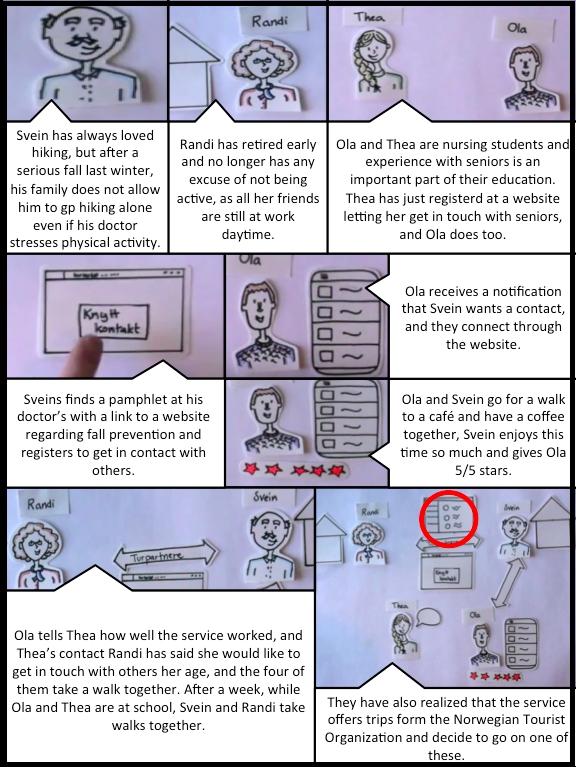
\includegraphics[width = 0.60\textwidth]{Figures/UserFilm1}
\caption{Story board of preliminary user story video}
    \label{fig:preVideo}
    \end{figure}

\chapter{Requirements}


\section{Use Cases}

\begin{figure}[H]
\centering
\includegraphics[width = 0.75\textwidth]{Figures/UseCase1}
\caption{Use case 1}
    \label{fig:UC1}
    \end{figure}

\begin{table}[H]
% See definition at beginning of main.
\begin{tabular}{ | L{0.25\linewidth} | L{0.75\linewidth} | } 
 \hline \rowcolor{lightgray}
 Use case 1 & User registration  \\ 
 \hline
 Actors & Customer, user \\ 
 \hline
 Stakeholders & Customers, developers users \\ 
  \hline
 Primary actor & user  \\ 
 \hline
 Pre-conditions & System is up and running \\ 
 \hline
 Post-conditions & The user has registered a profile and is logged in \\ 
  \hline
 Triggers & User visits the website and clicks to register \\ 
 \hline
Flow &
\vspace{-5mm}
    \begin{enumerate}[noitemsep]
  \item User enters the webpage.
  \item User navigates mouse to register button and clicks
  \item User fills in user information and submits the data
  \item The user has now created a profile and is logged in
   \end{enumerate}\\ 
 \hline
 Main success scenarios & User now has a profile registered and can use it to log in in the future \\ 
 \hline
 Alternative paths & 3a. User fails to register\\
 \hline
\end{tabular}
\caption{Use Case 1}
\end{table}

\begin{figure}[H]
\centering
\includegraphics[width = 0.75\textwidth]{Figures/UseCase2}
\caption{Use case 2}
    \label{fig:UC2}
    \end{figure}

\begin{table}[H]
\begin{tabular}{ | L{0.25\linewidth} | L{0.75\linewidth} | } 
 \hline \rowcolor{lightgray}
 Use case 2 & User log in  \\ 
 \hline
 Actors & Customer, user \\ 
 \hline
 Stakeholders & Customer, developers, user \\ 
  \hline
 Primary actor & User  \\ 
 \hline
 Pre-conditions & User has a registered a profile \\ 
 \hline
 Post-conditions & User has successfully logged in \\ 
  \hline
 Triggers & User clicks on the login button on the website  \\ 
 \hline
Flow & 
    \vspace{-5mm}
    \begin{enumerate}[noitemsep]
  \item User enters the webpage.
  \item User navigates mouse to log in button and clicks
  \item User fills in user information and clicks login
  \item The user has now logged in
   \end{enumerate}\\ 
 \hline
 Main success scenarios & User is now logged in and can use the service as a registered user \\ 
 \hline
 Alternative paths & 3a. The login fails\\
 \hline
\end{tabular}
\caption{Use Case 2}
\end{table}

\begin{figure}[H]
\centering
\includegraphics[width = 0.75\textwidth]{Figures/UseCase3}
\caption{Use case 3}
    \label{fig:UC3}
    \end{figure}

\begin{table}[H]
\begin{tabular}{ | L{0.25\linewidth} | L{0.75\linewidth} | } 
 \hline \rowcolor{lightgray}
 Use case 3 & User invites friend to self-created event  \\ 
 \hline
 Actors & Customer, user, other users \\ 
 \hline
 Stakeholders & Customer, developers, user, other users \\ 
  \hline
 Primary actor & User  \\ 
 \hline
 Pre-conditions & User is logged in and ready to create event \\ 
 \hline
 Post-conditions & User created an event and invited friends to it \\ 
  \hline
 Triggers & A button to create event is clicked after all the necessary information is submitted  \\ 
 \hline
Flow & 
    \vspace{-5mm}
    \begin{enumerate}[noitemsep]
  \item Click create new event button
  \item The user fills in relevant information for the event and clicks create
  \item The user searches for friends in their friends list and invites friends to his newly created event
   \end{enumerate}\\ 
 \hline
 Main success scenarios & An event is successfully created and friends are invited to it \\ 
 \hline
 Alternative paths & 2a. The user fails to register the event.
3a. The user does not manage to invite any friends.\\
 \hline
\end{tabular}
\caption{Use Case 3}
\end{table}

\begin{figure}[H]
\centering
\includegraphics[width = 0.75\textwidth]{Figures/UseCase4}
\caption{Use case 4}
    \label{fig:UC4}
    \end{figure}

\begin{table}[H]
\begin{tabular}{ | L{0.25\linewidth} | L{0.75\linewidth} | } 
 \hline \rowcolor{lightgray}
 Use case 4 & User downloads the app  \\ 
 \hline
 Actors & Customer, user \\ 
 \hline
 Stakeholders & Customer, developers, user \\ 
  \hline
 Primary actor & User  \\ 
 \hline
 Pre-conditions & User has a smart phone/tablet \\ 
 \hline
 Post-conditions & User successfully downloaded the app \\ 
  \hline
 Triggers & The user navigates to the “download app” page and follows the link to their preferred app store.  \\ 
 \hline
Flow & 
   \vspace{-5mm}
    \begin{enumerate}[noitemsep]
  \item User is on the web page and clicks the download app tab
  \item The user navigates to the preferred app store from the links provided
  \item Downloads the app
   \end{enumerate}\\ 
 \hline
 Main success scenarios & The app is downloaded to the user’s device \\ 
 \hline
 Alternative paths & 2a. The app store is down or not available \\
 & 3a. The user is unable to download the app\\
 \hline
\end{tabular}
\caption{Use Case 4}
\end{table}

\begin{figure}[H]
\centering
\includegraphics[width = 0.75\textwidth]{Figures/UseCase5}
\caption{Use case 5}
    \label{fig:UC5}
    \end{figure}

\begin{table}[H]
\begin{tabular}{ | L{0.25\linewidth} | L{0.75\linewidth} | } 
 \hline \rowcolor{lightgray}
 Use case 5 & User creates event  \\ 
 \hline
 Actors & Customer, user \\ 
 \hline
 Stakeholders & Customer, developers, user \\ 
  \hline
 Primary actor & User  \\ 
 \hline
 Pre-conditions & User is logged in \\ 
 \hline
 Post-conditions & User created event \\ 
  \hline
 Triggers & The user clicks create event button  \\ 
 \hline
Flow & 
    \vspace{-5mm}
    \begin{enumerate}[noitemsep]
  \item User is on the web page and is logged in and navigates to the dashboard
  \item User clicks the create event button 
  \item User fills in information about the event and clicks submit
   \end{enumerate}\\ 
 \hline
 Main success scenarios & The user has successfully created a new event. \\ 
 \hline
 Alternative paths & 3a. User fails to create event\\
 \hline
\end{tabular}
\caption{Use Case 5}
\end{table}

\begin{figure}[H]
\centering
\includegraphics[width = 0.5\textwidth]{Figures/UseCase6}
\caption{Use case 6}
    \label{fig:UC6}
    \end{figure}

\begin{table}[H]
\begin{tabular}{ | L{0.25\linewidth} | L{0.75\linewidth} | } 
 \hline \rowcolor{lightgray}
 Use case 6 & User adds friend to network  \\ 
 \hline
 Actors & Customer, user \\ 
 \hline
 Stakeholders & Customer, developers, user \\ 
  \hline
 Primary actor & User  \\ 
 \hline
 Pre-conditions & User is logged in \\ 
 \hline
 Post-conditions & User added friend to their network \\ 
  \hline
 Triggers & The user clicks search for other users button  \\ 
 \hline
Flow & 
    \vspace{-5mm}
    \begin{enumerate}[noitemsep]
  \item User in on the web page and navigates to the search bar
  \item User clicks the search to initiate the search
  \item User finds the person it wants to add and clicks add to friends list
   \end{enumerate}\\ 
 \hline
 Main success scenarios & The user has successfully added a person to their network \\ 
 \hline
 Alternative paths & 3a. User fails to add contact to their friends list\\
 \hline
\end{tabular}
\caption{Use Case 6}
\end{table}


\section{Functional Requirements}
Based on the use cases, we settled on the following functional requirements: 
\begin{center}
\begin{table}[H]
    \centering
\begin{tabular}{ |C{0.05\linewidth}|C{0.1\linewidth}|C{0.15\linewidth}|L{0.7\linewidth}| } 
 \hline \rowcolor{lightgray}
 \multicolumn{4}{|c|}{Functional Requirements} \\
 \hline
 No. & Priority & Use case no. & Description \\
 \hline
 F1 & P1 & UC1 & Register user profile \\ 
 \hline
 F2 & P1 & UC2 & Registered user should be able to login \\ 
  \hline
 F3 & P3 & UCX & Registered user should be able to edit their profile \\
  \hline
 F4 & P1 & UC3 & Registered user can create event \\
  \hline
 F5 & P1 & UC3 & Registered user can search for events \\
  \hline
 F6 & P1 & UC3 & Registered user can invite friends to event \\
  \hline
 F7 & P1 & UCX & Registered user can join others events \\
  \hline
 F8 & P2 & UCX & Non-registered user can view public events \\
  \hline
 F9 & P2 & UCX & Registered user can view their fitness information in his/her profile page \\
  \hline
 F10 & P2 & UC5  & Registered user can manually add their activities \\
  \hline
 F11 & P1 & UC3  & Registered user can search for and view other users’ profiles \\
  \hline
 F12 & P2 & UC3  & Registered user can view friend list \\
  \hline
 F13 & P2 & UCX  & Registered user can add/delete friends from friend list \\
  \hline
 F14 & P3 & UCX  & Registered users can instant message other users \\
  \hline
 F15 & P1 & UC4  & All users should be able to download the app from the website \\
  \hline
 F16 & P3 & UCX  & All users should be able to view different exercises on the web page \\
  \hline
 F17 & P3 & UCX  & All users should be able to take a simple fitness test on the web site\\
  \hline
 F18 & P2 & UCX  & Registered users should get updates from other users in a news feed \\
  \hline
 F19 & P2 & UCX  & All users should be able to get basic information about fall risk \\
 \hline
\end{tabular}
\caption{Functional Requirements}
 \label{table:funcReq}
\end{table}
\end{center}


\section{Non-Functional Requirements}

\begin{table} [H]\centering
    \begin{tabular}{ |C{0.05\linewidth}|C{0.15\linewidth}|L{0.7\linewidth}| } 
 \hline \rowcolor{lightgray}
 \multicolumn{3}{|c|}{Non-Functional Requirements} \\
 \hline
 No. & Name & Description \\
 \hline
 NF1 & Usability & As the service is designed with the elderly in mind, simple and easily understandable interfaces is a must \\ 
 \hline
 NF2 & Security & Secure personal data like username, password, email and fitness information \\ 
  \hline
 NF3 & Accessibility & The users should be able to access the system \\
  \hline
 NF4 & Availability & The system is up and running at all times \\
  \hline
 NF5 & Maintainability & Clean and concise code that can be maintained and extended easily if needed. \\
  \hline
 NF6 & Performance & The system must be fast and responsive \\
 
 \hline
\end{tabular}
\caption{Non-Functional Requirements}
\end{table}

\section{Changes in Requirements(Change Order?)}
\subsection{Additions}
\begin{enumerate}
    \item Users of the system should be distinguished between administrators and non-administrators.
    \item Administrators must be able to create user accounts
    \item Administrators must be able to create exercises
    \item Administrators must be able to enter personal data about users
    \item Users must be able to select exercises and add them to their accounts
    \item Users must be able to add exercises to events
\end{enumerate}

\subsection{Removals}
Only one functional requirement was removed halfway through the project. This was 
\begin{enumerate}
    \item F8: \textit{Non-registered users can view public events}
    \begin{itemize}
        \item[-] Replaced by public events only being visible to registered users.
    \end{itemize}
\end{enumerate}
 
No other functional requirements were removed, but parts of the functionality in the original requirements were replaced with placeholders in the final system. This was in agreement with the customer, as the ADAPT project was not able to deliver the necessary data needed to implement the functionality. The requirements affected were: 
\begin{enumerate}
    \item  F9: \textit{Users can view their own fitness information.} The fitness information should have consisted of diagrams and graphs and a composite indicator displaying the general fitness based on several different parameter. Since it never became clear which parameters would form the basis for this fitness indicator, the final solution contains a placeholder fitness indicator, but no functionality is attached to this indicator. 
    \item F17: \textit{Take a simple fitness test.} The fitness test is also a placeholder test. The parameters necessary for creating a trustworthy test were never supplied.
    
\end{enumerate}


\section{Requirements Evaluation??}

// Should we include a section on Requirements Evalutation?




\chapter{Alternative Solutions}
\section{Evaluation of Existing Solutions}
Seven different web solutions addressing fall risk prevention were evaluated according to set criteria based on the functional requirements of the project. Firstly, positive and negative aspects of the individual cites were summarized and then a matrix was construced, see Table \ref{table:evaluationMatrix}, summarizing how all the different cites fufilled the pre-defined requiremtns.
\subsection{Evaluation Criteria}
In order to evaluate the different solutions, the most characteristic functional requirements of the desired solution were selecetd. The selected requiremetnts were (for full description of functional requirements see Table \ref{table:funcReq}):

F1: Register user profile

F4: Log in functionality for users 

F6: Invite friends to events 

F9: View personal fitness information

F13: Add friends to personal network

F15: Download app(s)

F16: View exercises

F17: Take a fitness test

F19: Basic information about fall risk


\subsection{Sindre 1}
\begin{center}
\begin{tabu} to 0.8\textwidth{ |X[l]|X[l]| } 
\hline \rowcolor{lightgray}
Pros & Cons \\
\hline
Pro1 & 
Con2 \\ 
\hline
Pro2 & Con2 \\ 
\hline

\end{tabu}
\end{center}

\subsection{Sindre 2}
\begin{center}
\begin{tabu} to 0.8\textwidth{ |X[l]|X[l]| } 
\hline \rowcolor{lightgray}
Pros & Cons \\
\hline
Pro1 & 
Con1 \\ 
\hline
pro2 & Con2 \\ 
\hline

\end{tabu}
\end{center}

\subsection{Fallforebygging.no}
Fallforebygging.no \cite{fallforebygging} is a Norwegian website dedicated to preventing falls. It is an extensive website with content ranging from Causes and Consequences to  Prevention methods, and includes videos, information about lectures and links to more information. 
\begin{center}
\begin{tabu} to 0.8\textwidth{ |X[l]|X[l]| } 
\hline \rowcolor{lightgray}
Pros & Cons \\
\hline
Include much statistics about fall risk & 
The website has a image of a fall on the main page. Our customer clearly wants us to not feed into the stigmas regarding old age and health \\ 
\hline
Specific section on causes and methods of prevention & Negative statistics \\ 
\hline
\end{tabu}
\end{center}

\subsection{Stopfalls.org}
This is the website of Fall Prevention Center of Excellence based in California. Their mission is: 
\begin{center}
\begin{tabu} to 0.8\textwidth{ |X[l]|X[l]| } 
\hline \rowcolor{lightgray}
Pros & Cons \\
\hline
The site offers brochures with exercise programs to prevent falls. They appear inspiring and include positive images. The downside is that they are not free & 
The geographical connection of the site is unsuitable for our purposes. It offers link to several California based services, which naturally are of no importance to Norwegian seniors.  \\ 
\hline
The site has a DVD with more exercises one can do at home to prevent falls, but this DVD is not free either.
 & The language of the site of naturally an obstacle, but the development team can nonetheless  use the site as inspiration. \\ 
\hline
\end{tabu}
\end{center}

\subsection{Dytt.no}
\begin{center}
\begin{tabu} to 0.8\textwidth{ |X[l]|X[l]| } 
\hline \rowcolor{lightgray}
Pros & Cons \\
\hline
The activities fit everyone and they are easy &
The service focuses on businesses, not private persons \\ 
\hline
Provides health benefits & The service is not free \\ 
\hline
\end{tabu}
\end{center}

\subsection{Endomondo.no}
\begin{center}
\begin{tabu} to 0.8\textwidth{ |X[l]|X[l]| } 
\hline \rowcolor{lightgray}
Pros & Cons \\
\hline
Pro1 & 
TCon1 \\ 
\hline
Pro2 & Con2 \\ 
\hline
\end{tabu}
\end{center}

\subsection{Summary}
\begin{center}
\begin{table} [!h] \centering
    \begin{tabular}{@{} cl*{10}c @{}}
        & & \multicolumn{10}{c}{Websites} \\[2ex]
        & & \rot{Sinde1} & \rot{Sindre2} & \rot{Fallforebygging.no} & \rot{Stopfalls.org} 
        & \rot{Dytt.no} & \rot{Endomondo}  & \rot{Facebook} \\
        \cmidrule{2-9}
        & F1              & ? & ? &     &     & \OK & \OK &  \OK\\
        & F4              & ? & ? &     &     & \OK &     &  \OK\\
        & F6              & ? & ? &     &     & \OK &     &  \OK\\
        & F9              & ? & ? &     &     & \OK & \OK &     \\
        & F13             & ? & ? &     &     & ?   & \OK &  \OK\\
        & F15             & ? & ? & \OK &     &     & \OK &  \OK\\
        & F16             & ? & ? &     & \OK &     & \OK &     \\
        & F17             & ? & ? &     &     &     & \OK &     \\
        & F19             & ? & ? & \OK & \OK &     &     &     \\
 \rotvert{\rlap{~Functional Requirements}}
        & Comments                &  &   &   &   &   &   &    \\
        \cmidrule[1pt]{2-9}
    \end{tabular}
    \caption{Evaluation of Existing Solutions}
    \label{table:evaluationMatrix}
\end{table}
\end{center}

\chapter{Desired Solution}
\section{User Story Video}
Based on the functional requirements, and after receiving inspiration form evaluating existing solutions, the team came up with a design suggestion together with the customer. To present the vision we had of what a solution could look like, the team created a user story video \cite{video} in which several scenarios of interacting with the solution where presented. The video also explained how the different users came into contact with the solution and why they begun using it. The story line of the video can be seen here, Figure \ref{fig:video}, with images from the video depicting the most important use cases of the solution. 

\begin{figure}[H]
\centering
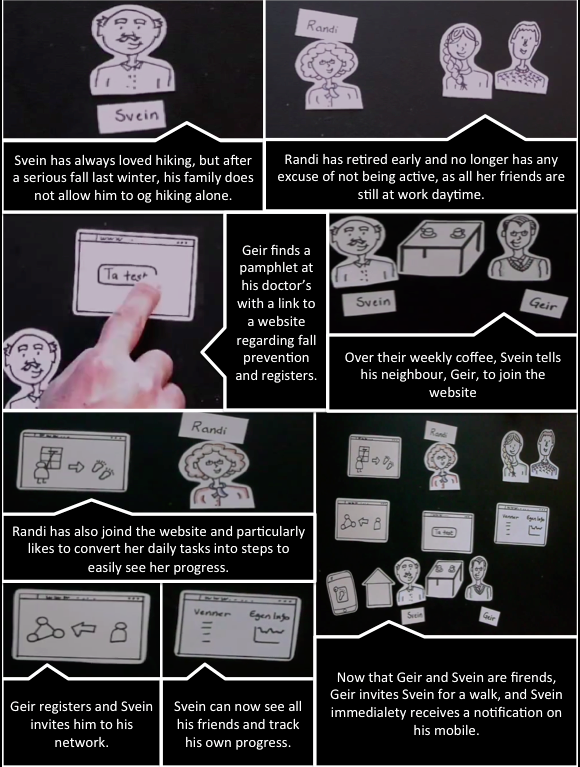
\includegraphics[width = 0.75\textwidth]{Figures/VideoImages}
\caption{Story board of user story video}
    \label{fig:video}
    \end{figure}

\section{Wireframes}
Moving on from the concept displayed in the video, the team made wireframes and mock-ups to display the initial ideas of what the solution could look like. This is how we initially envisioned the system: 


\begin{figure}[H]
\centering
 \textbf{Web-based Solution}\par\medskip
\begin{subfigure}{.5\textwidth}
  \centering
  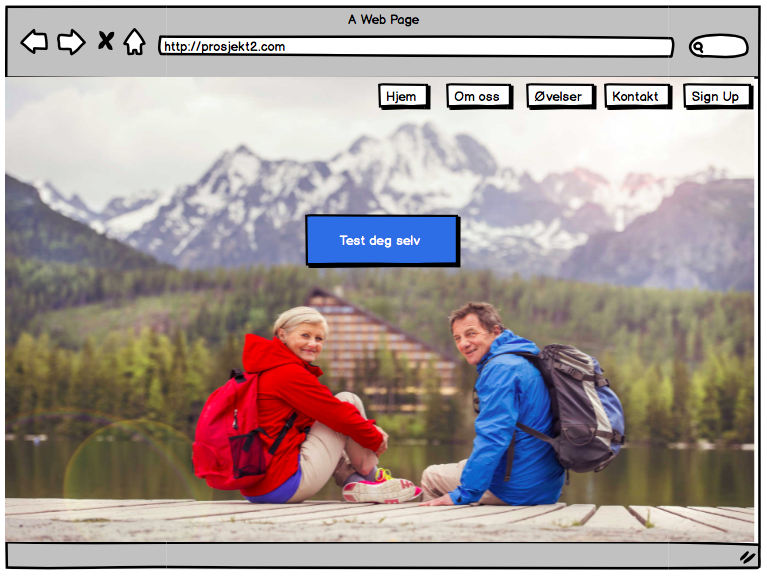
\includegraphics[width=.8\linewidth]{wireframes/web/Home}
  \caption{Home page of web application, where the test is the focal point.}
  \label{fig:videoHome}
\end{subfigure}%
\begin{subfigure}{.5\textwidth}
  \centering
  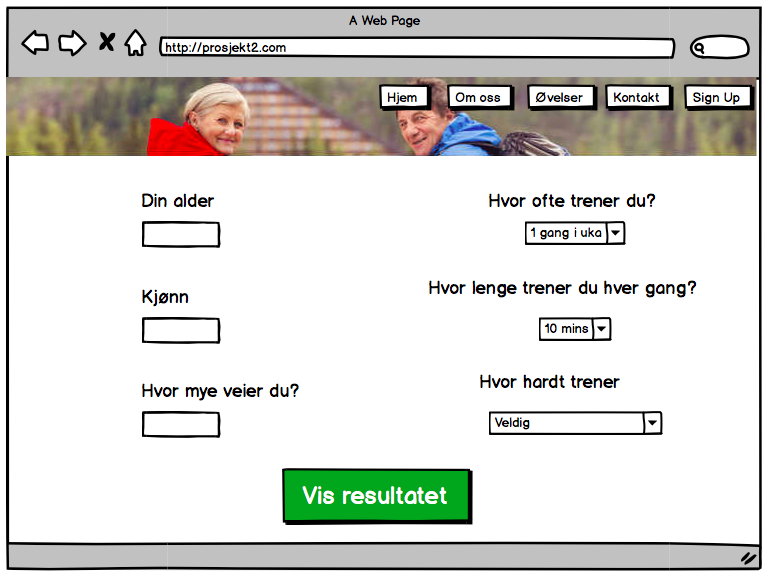
\includegraphics[width=.8\linewidth]{wireframes/web/TestDetails}
  \caption{Test interface}
  \label{fig:videoTest}
\end{subfigure}\\
\break
\begin{subfigure}{.5\textwidth}
  \centering
  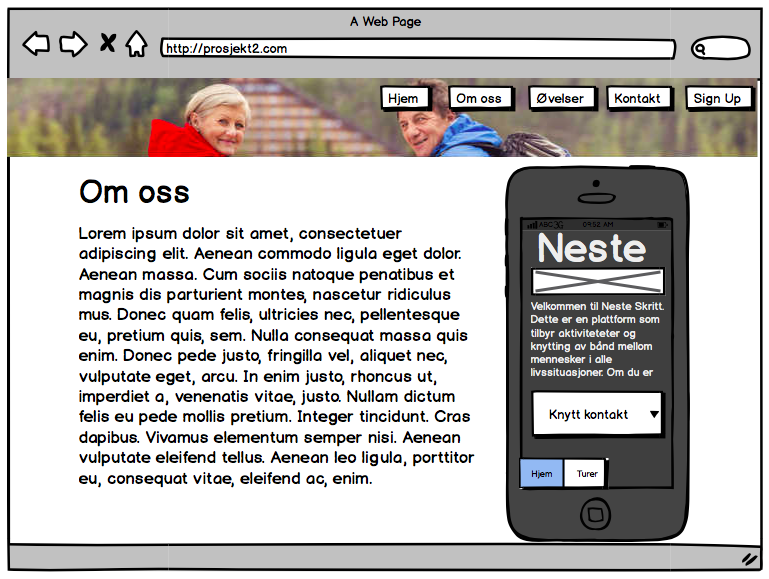
\includegraphics[width=.8\linewidth]{wireframes/web/About}
  \caption{About Us page. If the name was changed to info, this page could also serve as the source of information about fall risk and prevention.}
  \label{fig:videoAbout}
\end{subfigure}%
\begin{subfigure}{.5\textwidth}
  \centering
  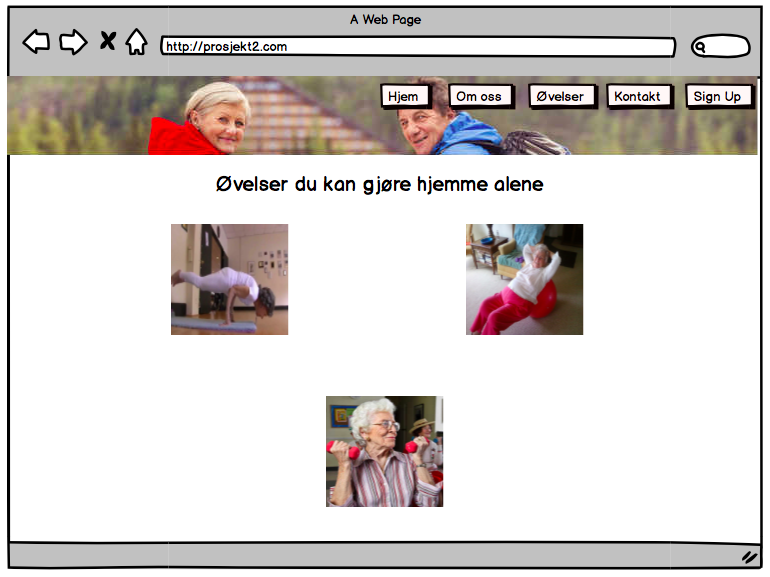
\includegraphics[width=.8\linewidth]{wireframes/web/Activities}
  \caption{Activities page: the different activities are displayed here.}
  \label{fig:videoACtivities}
\end{subfigure}\\
\break
\begin{subfigure}{.5\textwidth}
  \centering
  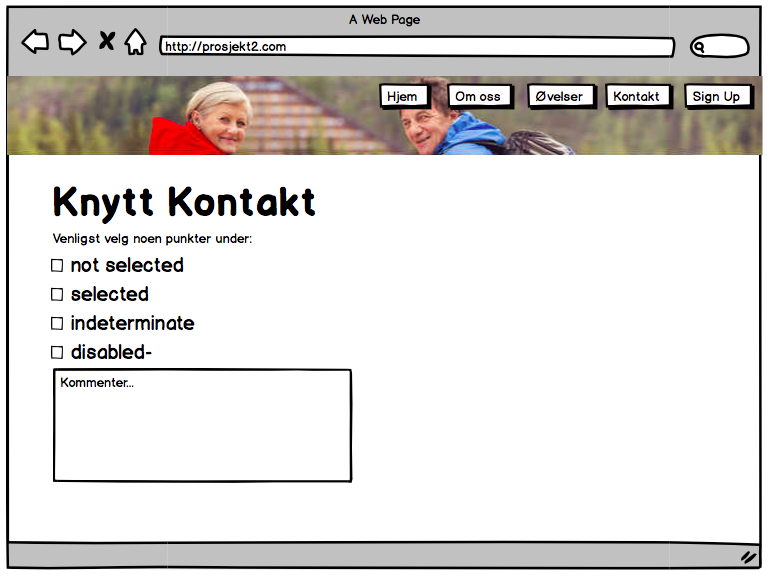
\includegraphics[width=.8\linewidth]{wireframes/web/Contact}
  \caption{Contact: a page where one can make acquaintances without necessarily registering to the service. }
  \label{fig:videoContact}
\end{subfigure}%
\begin{subfigure}{.5\textwidth}
  \centering
  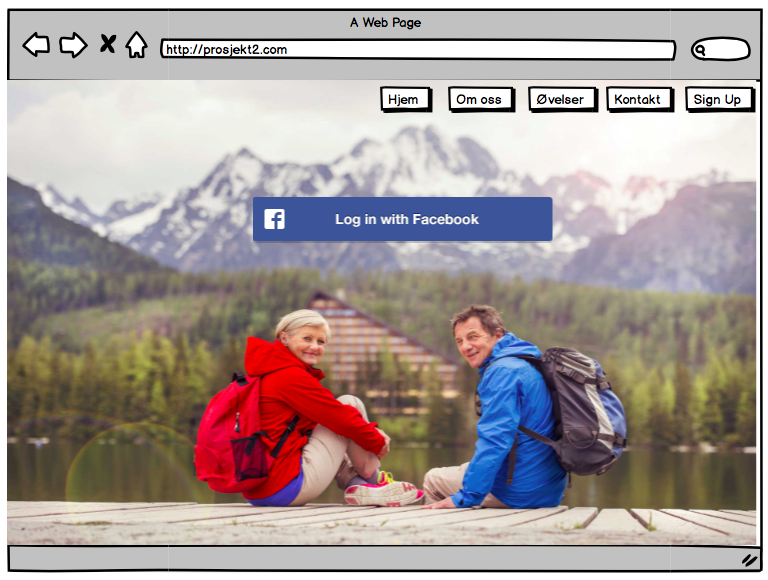
\includegraphics[width=.8\linewidth]{wireframes/web/SignUp}
  \caption{SignUp page: here users can sign in with Facebook to avoid long registration forms. The final solution could possibly include google-signIn as well, and perhaps a custom registration for  for users with none of the above-mentioned accounts.}
  \label{fig:videoSignUp}
\end{subfigure}
\caption{Wireframes for web solution}
\end{figure}

    

\begin{figure}[H]
\centering
 \textbf{Mobile Application}\par\medskip
\begin{subfigure}{.5\textwidth}
  \centering
  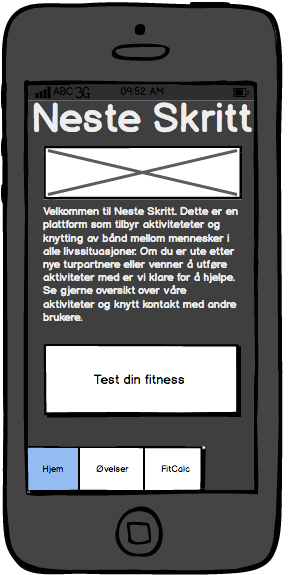
\includegraphics[width=.5\linewidth]{wireframes/app/Home}
  \caption{Home page}
  \label{fig:appHome}
\end{subfigure}%
\begin{subfigure}{.5\textwidth}
  \centering
  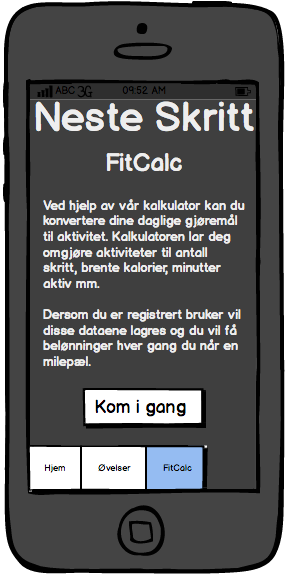
\includegraphics[width=.5\linewidth]{wireframes/app/Test}
  \caption{Test page}
  \label{fig:appTest}
\end{subfigure}\\
\begin{subfigure}{.5\textwidth}
  \centering
  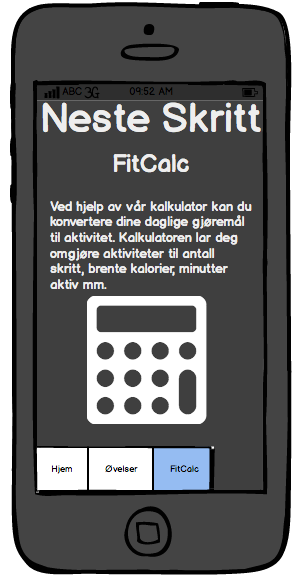
\includegraphics[width=.5\linewidth]{wireframes/app/Calc}
  \caption{Activity converter}
  \label{fig:appCalc}
\end{subfigure}\\
\begin{subfigure}{.5\textwidth}
  \centering
  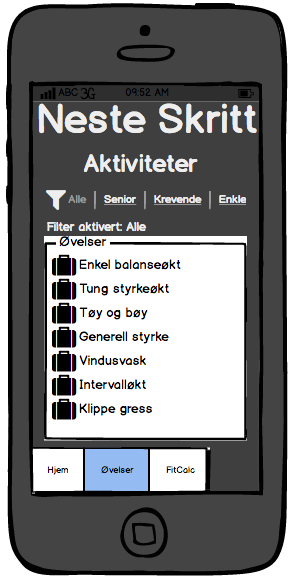
\includegraphics[width=.5\linewidth]{wireframes/app/Activities}
  \caption{Activities page}
  \label{fig:appActivities}
\end{subfigure}%
\begin{subfigure}{.5\textwidth}
  \centering
  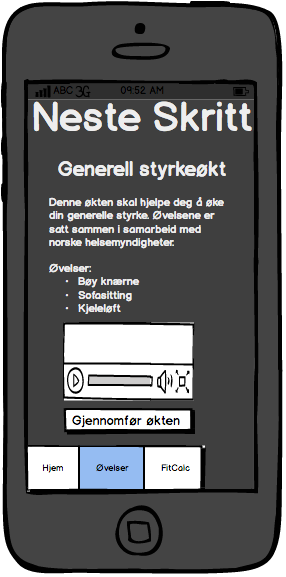
\includegraphics[width=.5\linewidth]{wireframes/app/Activity}
  \caption{Page for displaying an individual activity}
  \label{fig:appActivity}
\end{subfigure}
\caption{Wireframes for mobile application}
\end{figure} 




\chapter{Project Management}


\section{Choice of Process Model}
A strict Scrum based approach to software development was required by the product owner in this project. In addition, the two principles \textit{decide as late as possible} and \textit{deliver as fast as possible}  from  LEAN software development were emphasised by the product owner. The development team had weekly meetings with the product owner and, thus, chose to structure the project in one-week long sprints. 

An agile approach to software development, coupled with short sprints were, in this project, essential to be able to accommodate the product owner's focus on the two Lean principles mentioned above. A more traditional plan-based approach would have forced both the customer and the development team to make decisions at a very early stage. 

Much of the communication between the product owner and the development team was based on pitching new ideas and solutions. This process relied heavily on mockups and wireframes, and the agile approach enabled us to easily present solutions at every stage of the development life cycle.


\subsection{Customer Meetings}
Every Thursday, the group met with the product owner for sprint retrospective and planning. During these meetings, the development team began with presenting a demo of the most recent version of the system to the product owner. Based on the feedback of the product owner, we settled on which features to keep, which to discard and which to develop further. This then lead us to the sprint planning of the next sprint, where we decided which features should be included in the next version of the product. 

The customer strongly practiced the Lean principle of \textit{decide as late as possible}, and this was an aspect of the development process unfamiliar to most of the team members. As the development team could not, form the start, neither rely on, nor elicit a fixed list of requirements, these weekly meetings were essential to prevent stagnation of the development. 

\subsection{Supervisor Meetings}
In addition to weekly meetings with the product owner for the development of the solution, the team also had bi-weekly meetings with our course supervisor, Soudabeh Khodambashi, to ensure our progress with the course as a whole. Prior to the meetings we submitted status reports to enable the supervisor to follow our progress and make her aware of any difficulties we might be experiencing. The status report gave a detailed overview of what we had done during the last meeting, what were our plans for the coming sprints, and any difficulties, coupled with an updated risk analysis.

\vspace{10mm}

//Should we include an example of a status report in the appendix? 
Ex: An example of a status report can be found in Appendix XX, figure XX.
% Status report link needed !

\section{Time Constraints and Work Breakdown Structure}

As stated in the course description, the workload of the course is expected to be approximately 20 hours per week. Thus, the group used this as a guiding estimate when calculating the time constraints of the project. We are 7 members on the team which led to 140 hours available each week, and taking into consideration holidays, we arrived at this estimate, Table \ref{table: Time}: 


\begin{table}[H]
\centering
\begin{tabu} to 0.8\textwidth{ |X[l]|X[l]|X[L]| } 
\hline \rowcolor{lightgray}
Months & Weeks & Hours  \\
\hline
Jan &  &  \\ 
\hline
Feb & 4 & 560\\ 
\hline
March & 3.5 & 490\\
\hline
April  & 4 & 560\\
\hline
May & 1 & 140\\
\hline
\textbf{Total} & & \textbf{1750}\\
\hline
\end{tabu}
\caption{Time Constraints}
\label{table: Time}
\end{table}

The groups were announced on Jan 21st, and the following week was spent meeting the group and having the initial customer meeting. Thus, no weeks in January were included in the time estimate of the project.
The term ends in April and, thus, only one week is allocated in May, primarily to finish up the report.

Following the initial meetings with the customer, the group decided on a work breakdown structure (WBS) for the project, see Figure \ref{fig:WBS}, and assigned percentages to the different sections. 
 
\begin{figure}[H]
\centering
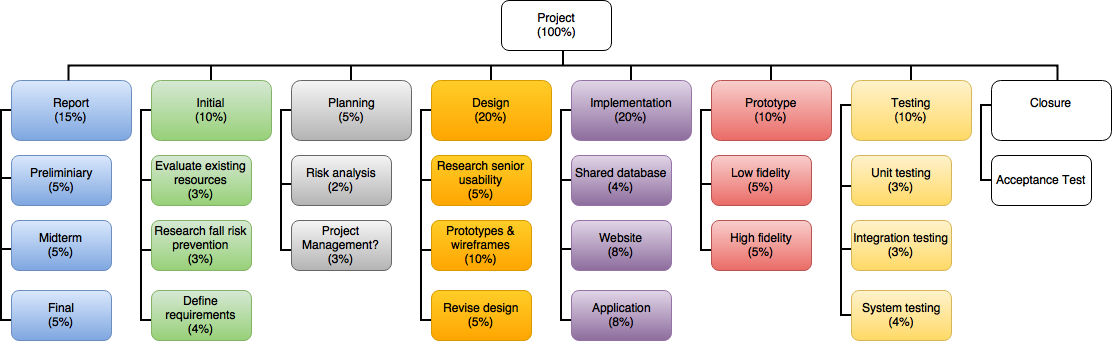
\includegraphics[scale=0.4]{Figures/WBS.png}
\caption{WBS}
\label{fig:WBS}
\end{figure}

Further, based on the WBS diagram and time constraints, we calculated how many hours we had available for each section which laid the foundation for project management. The allocation of hours on different aspects of the project can be seen in Table \ref{table: AllocatedTime}. 

\begin{table}[H]
\centering
\begin{tabu}{ |m{9em}|m{15em}|m{3em}|} 
\hline \rowcolor{lightgray}
Sections & Subsections & Hours\\
\hline
\multirow{3}{*}{Report 262.5h} & Preliminary & 87.5 \\

& Midterm & 87.5\\

& Final & 87.5\\
\hline
\multirow{3}{*}{Initial 175h} & Evaluate existing resources & 52.5\\
& Research fall risk prevention & 52.5\\
& Define requirements & 70\\
\hline
\multirow{2}{*}{Planning 87.5h} & Risk analysis & 35\\
& Project management & 52.5 \\
\hline
\multirow{3}{*}{Design 350h} & Research senior usability & 87.5\\
& Prototype and wireframes & 175\\
& Revise design & 175 \\
\hline
\multirow{3}{*}{Implementation 350h} & Shared database & 350\\
& Website & 140\\
& Application & 140 \\
\hline
\multirow{2}{*}{Prototype 175h} & Low fidelity & 175\\
& High fidelity & 175\\
\hline
\multirow{3}{*}{Testing 175h} & Unit testing & 52.5\\
& Integratiog testing & 52.5 \\
& System testing & 70 \\
\hline
\end{tabu}
\caption{Time allocated to different aspects of project}
\label{table: AllocatedTime}
\end{table}


\section{Risk Analysis}
Managing risk is essential to a software project and a meeting to analyse the risks was settled early. Firstly, in the \textit{risk identification} process, the team identified potential risks and organized them into several larger categories: requirements, team, planning and technical. Secondly, during \textit{risk analysis}, the team estimated both the likelihood and potential impact of each risk. This was done by awarding a number ranging from 1-9 where 1 indicates low likelihood and impact, and 9 indicates high likelihood and impact. Thirdly, the team identified actions to prevent and mitigate the risks during the \textit{risk planning} phase. The outcome of these three first phases is a risk assessment matrix, see Figure \ref{fig:RiskFull} in the appendix. The matrix lists all the risks accompanied by the likelihood and impact estimates along with preventative and mitigative actions. Below follows a condensed version of the risk assessment matrix, Figure \ref{fig:Risk}, giving a quick overview of how severe the different risks are, with R1, R2, R3, etc referring to Risk 1, Risk 2, Risk 3 and so on. The explanations of each risk can be found in the appendix, Figure \ref{fig:RiskFull}.
\begin{figure}[h!]
\centering
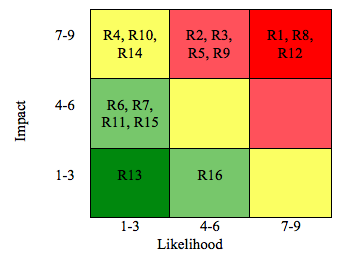
\includegraphics[scale=0.8]{Figures/RiskAnalysis.png}
\caption{Risk Analysis}
\label{fig:Risk}
\medskip
\small
R1, R2, R3, etc refers to Risk 1, Risk 2, Risk 3 and so forth, of the extended risk analysis matrix, see Figure \ref{fig:RiskFull} in the appendix.
\end{figure}

Lastly,  the team decided to perform \textit{risk monitoring} by regularly assessing the risks and revising the risk analysis matrix when needed. 


\section{Project Management Tools}
\subsection{GitHub}
In addition to the source code management provided by git, using gitHub lets us share the repository with all the team members while at the same time providing several project management features including backlog management, task management, sprint organization and easy communications with the customer. Having code and project management features in the same place eases collaboration as all team members then know where to look for new tasks, and the state of the product. We were not aware of all of these features of GitHub at the beginning of the project and, only towards the end of the project, did the team switch to using gitHub's project management features. 
\subsection{Trello}
Trello is a tool to help people collaborate and organizes your projects into boards. At a glance Trello shows you what is being worked on, who is working on what and what remains to be done. 
As we, as a team,  do not have office space or an alternative fixed location to work from, we do not have a suitable place for a physical Scrum board. Trello is  thus an online alternative to the Scum board which shows the current status for the project, or at least the sprint.
\subsection{Google Docs}
Google Drive is a file storage and synchronization service that allows users to store files in the cloud, share files, and edit documents, spreadsheets, and presentations with collaborators. It is essential for our team that everyone in the team has the same access to documents relating to the project, and are able to contribute to them.
\section{Group Communication Tools}
\subsection{Slack}
Slack is a cloud-based team collaboration tool used for communication through different chat rooms and channels. We use slack for communication within the team. Slack also has an app which gives you  instant notifications if a group member post anything in one of the channels. Thus, this communication tool is therefore more suitable than for instance email communications as it allows more instant communication. It is also better suited to this project than Facebook, as it allows us to structure our communication into different channels. 

\section{Deviations}

The concept refining phase took much longer time that the team had initially anticipated, with the result of coding being postponed. However, the long concept refining phase, was one of the main focus points of the customer in the early stages. This led to us having more sprints devoted to wireframing than was initially planned, and thus implementation was pushed back. The product owner, however, was pleased with this line of development of rapid prototyping and did not seem to be dissatisfied with the fact that coding was postponed. Consequently, we do not consider the project to be delayed as a result of the coding delay.
\\\\
We also encountered some difficulties with eliciting requirements from the product owner. It appeared to us that the product owner often focused on what was to be accomplished by the next sprint, and we found it difficult to settle on a long term plan. Thus, no milestones for the whole project were decided upon, nor did we settle on a release plan. It was made clear that user testing would be an integral part of the project, but although we had a meeting to plan the usability test, no dates were ever settled in this regard either. Thus, making a concrete time plan has been difficult. This issue is expanded on in Chapter \ref{lessons}. 
\\\\
Another deviation from the plan was related to our sprint management. Halfway into the project the product owner instructed us to switch to GitHub's issue list as a sprint backlog. Up to this point, we had been keeping track of our tasks using a spreadsheet in Google docs. The switch made it easier for the client to keep track of the tasks. He also stressed that it was important to keep the code close to the roadmap of the development process.

\section{Team Organization}
\subsection{Responsibilities}
All team members were part of coding and planning in the projects, but the following areas of responsibility were distributed among the team members:
\begin{itemize}
    \item[] \textbf{Emil S. Andersen:} Project leader, communication manager and documents manager
    \item[] \textbf{Christoffer Jahren:} Head of mobile division, responsible for developing the mobile version, both iOS and Android version of the app.
    \item[] \textbf{Eirik Wist:} Co-head of mobile division 
    \item[] \textbf{Sindre Berntsen:} Documentation and datamodelling 
    \item[] \textbf{Sarah Svedenbrog:} Scrum master and report
    \item[] \textbf{Brang Nu Bok Tong:} Webmaster: frontend and backend.
    \item[] \textbf{Alexander Foosnæs:} Test leader 
\end{itemize}
\subsection{Pair-Programming}
Although the team members were assigned tasks individually, pair-programming was used extensively. Most of the team members were unfamiliar with the frameworks we used in the project and the learning curve was steep. When one team members had learnt something, and another was going to do the same, the two often pair-programmed so that the time invested in learning by one team member could directly benefit another team members and, in turn, the team.

In addition to teaching other team members how to do certain tasks, pair-programming was also used for problem-solving. If one team member had been working a long time on a task and not succeeding in fulfilling it, he/she would often team up with another. Often problems were solved quickly in this way, and both team members involved benefited from the process.

\section{Sprints}
\subsection*{Sprint 1: Feb 5th - Feb 11th}
Table \ref{table: sprint1} is a summary of sprint 1. See Appendix \ref{sprint1} for complete breakdown of sprint 1. 

\begin{table}[H]

\begin{tabu} to 1.0\textwidth { | X[l] | X[l]| }
\hline\rowcolor{lightgray}
Objective of sprint & Summary of tasks completed\\
\hline
User story video & User story video\\
\hline
Wireframes of web solution & Wireframes of web solution\\
\hline
Wireframes of mobile application & Wireframes of mobile application\\
\hline
\end{tabu}
\caption{Summary of sprint 1}
\label{table: sprint1}
\end{table}


\subsection*{Sprint 2: Feb 11th -Feb 18th}
Table \ref{table: sprint2} is a summary of sprint 2. See Appendix \ref{sprint2} for complete breakdown of sprint 2. 
\begin{table}[H]
\begin{tabu} to 1.0\textwidth { | X[l] | X[l]| }
\hline\rowcolor{lightgray}
Objective of sprint & Summary of tasks completed\\
\hline
Senior usability research & Senior usability research\\
\hline
Fall prevention research & Fall prevention research\\
\hline
Evaluate existing solutions & Evaluate existing solutions\\
\hline
Elicit concrete requirements form customer & \\
\hline
\end{tabu}
\caption{Summary of sprint 2}
\label{table: sprint2}
\end{table}

Comments:  In this sprint, we begun having difficulties with eliciting clear requirements from the customer.


\subsection*{Sprint 3: Feb 18th - Feb 25th}
Table \ref{table: sprint3} is a summary of sprint 3. See Appendix \ref{sprint3} for complete breakdown of sprint 3. 
\begin{table}[H]
\begin{tabu} to 1.0\textwidth { | X[l] | X[l]| }
\hline\rowcolor{lightgray}
Objective of sprint & Summary of tasks completed\\
\hline
Revised user story film & Revised user story film\\
\hline
Revised mockups & Revised mockups\\
\hline
Research technologies & Research technologies\\
\hline
\end{tabu}
\caption{Summary of sprint 3}
\label{table: sprint3}
\end{table}

Comment: This sprint was largely concerned with revising the concept for the solution and much time was spent updating mockups and the user story film.

\subsection*{Sprint 4: Feb 25th - March 3rd}
Table \ref{table: sprint4} is a summary of sprint 4. See Appendix \ref{sprint4} for complete breakdown of sprint 4. 
\begin{table}[H]
\begin{tabu} to 1.0\textwidth { | X[l] | X[l]| }
\hline\rowcolor{lightgray}
Objective of sprint & Summary of tasks completed\\
\hline
Installation manual & Installation manual\\
\hline
Download app from webpage & Download app from webpage\\
\hline
Set up database & Set up database\\
\hline
Create user profile & Create user profile without form validation\\
\hline
\end{tabu}
\caption{Summary of sprint 4}
\label{table: sprint4}
\end{table}

\subsection*{Sprint 5: March 3rd - March 10th }
Table \ref{table: sprint5} is a summary of sprint 5. See Appendix \ref{sprint5} for complete breakdown of sprint 5. 
\begin{table}[H]
\begin{tabu} to 1.0\textwidth { | X[l] | X[l]| }
\hline\rowcolor{lightgray}
Objective of sprint & Summary of tasks completed\\
\hline
Flowchart for website & Flowchart for website\\
\hline
Download app from webpage & Link to app on website\\
\hline
Fill placeholders on homepage with actual information & Fill placeholders on homepage with actual information\\
\hline
\end{tabu}
\caption{Summary of sprint 5}
\label{table: sprint5}
\end{table}

Comment: The html page for downloading the app was implemented, but actually downloading an app was pushed to the next sprint.

\subsection*{Sprint 6: March 10th - March 17th}
Table \ref{table: sprint6} is a summary of sprint 6. See Appendix \ref{sprint6} for complete breakdown of sprint 6. 
\begin{table}[H]
\begin{tabu} to 1.0\textwidth { | X[l] | X[l]| }
\hline\rowcolor{lightgray}
Objective of sprint & Summary of tasks completed\\
\hline
State diagram of website & State diagram of website\\
\hline
Register new user & Register new user\\
\hline
Research dashboard component & Research dashboard and web usability for seniors\\
\hline
\end{tabu}
\caption{Summary of sprint 6}
\label{table: sprint6}
\end{table}

Comment: Much time was spent working on the report in this sprints. Thus, our objectives focused more on research than implementing functionality.

\subsection*{Sprint 7: March 17th - April 14th}
Table \ref{table: sprint7} is a summary of sprint 7. See Appendix \ref{sprint7} for complete breakdown of sprint 7. 
\begin{table}[H]
\begin{tabu} to 1.0\textwidth { | X[l] | X[l]| }
\hline\rowcolor{lightgray}
Objective of sprint & Summary of tasks completed\\
\hline
Creating and displaying events & Events added to the database\\
\hline
Algorithms for newsfeed & Algorithms for newsfeed\\
\hline
Searchbar & Searchbar designed\\
\hline
\end{tabu}
\caption{Summary of sprint 7}
\label{table: sprint7}
\end{table}

\textbf{Comment:} As this sprint began just before Easter, the actual work began after Easter, and in order to be able to meet the customer and have a status update, we let this sprint last approximately two weeks. 

With the unfamiliar technology, creating and displaying events took much longer time than expected, and the tasks related to it were further broken down in later sprints.
The same applies to the functionality of the search bar.


\subsection*{Sprint 8: April 14th - April 21st}


Switched to sprint management on GitHub

Table \ref{table: sprint8} is a summary of sprint 8. See Appendix \ref{sprint8} for complete breakdown of sprint 8. 
\begin{table}[H]
\begin{tabu} to 1.0\textwidth { | X[l] | X[l]| }
\hline\rowcolor{lightgray}
Objective of sprint & Summary of tasks completed\\
\hline
Accept/decline invitations to events & Accept/decline invitations to events\\
\hline
Filter and sort events & Filter and sort events\\
\hline
Internationalizing text & \\
\hline
\end{tabu}
\caption{Summary of sprint 8}
\label{table: sprint8}
\end{table}

\textbf{Comment:} Making the text internationalized was postponed until the next sprint since the group member who was assigned to it was unexpectedly absent.

\subsection*{Sprint 9: April 21st - April 28th}
Table \ref{table: sprint9} is a summary of sprint 9. See Appendix \ref{sprint9} for complete breakdown of sprint 9. 
\begin{table}[H]
\begin{tabu} to 1.0\textwidth { | X[l] | X[l]| }
\hline\rowcolor{lightgray}
Objective of sprint & Summary of tasks completed\\
\hline
Update event & Update event\\
\hline
Admin view & Admin view\\
\hline
Bug fixing & Bug fixing\\
\hline
\end{tabu}
\caption{Summary of sprint 9}
\label{table: sprint9}
\end{table}

\subsection*{Sprint 10: April 28th - May 6th }
Table \ref{table: sprint10} is a summary of sprint 10. See Appendix \ref{sprint10} for complete breakdown of sprint 10. 
\begin{table}[H]
\begin{tabu} to 1.0\textwidth { | X[l] | X[l]| }
\hline\rowcolor{lightgray}
Objective of sprint & Summary of tasks completed\\
\hline
App integration & fill in what got done\\
\hline
App roadmap & fill in what got done\\
\hline
\end{tabu}
\caption{Summary of sprint 10}
\label{table: sprint10}
\end{table}

\textbf{Comment:} We're currently in this sprint, so we will fill it out once we are done.

\section{Gantt Chart}
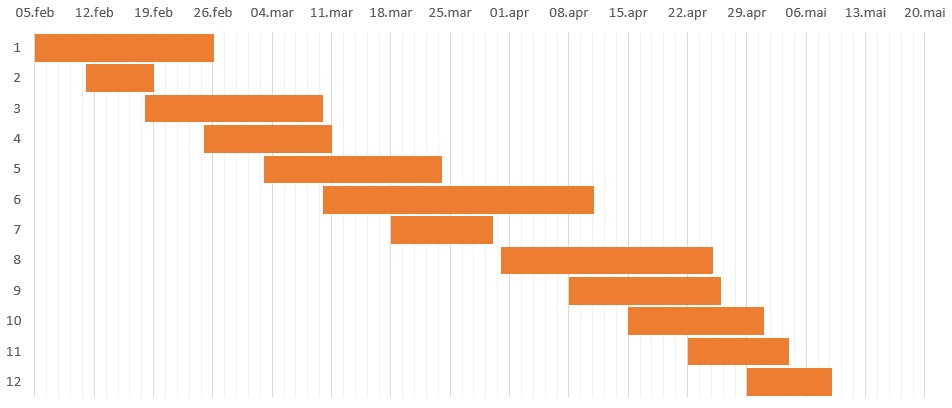
\includegraphics[width=1.0\textwidth]{Figures/Gantdiagram}

//The Gantt chart must be elaborated on here as an evaluation of all our sprints combined.

\chapter{Development Environment}
\section{Development Tools}
\subsection{Version Control - Git}
To manage different versions of our product code, we used the "free and open source distributed version control system "\cite{git} git. With seven team members working on the same code, the branching feature is especially important.
As many of the team members have limited experience with bigger software development projects, the fact that each team members has their own copy of the repository is a safety mechanism to prevent code corruption. Local repositories and branching allows team members to experiment with and test code, while not having to worry about corrupting the project. 
However, code corruption can always occur, and in the event of this, the use of git would make it unproblematic to restore the code to a working state. 
\subsection{Prototyping - Balsamiq Mock-ups}
Balsamiq mock-ups is a  graphical user interface mockup builder application. It allows the designer to arrange pre-built widgets using a drag-and-drop WYSIWYG editor to quickly and easily create mockups and wireframes. A large part of this project concerns itself with coming up with concepts of how to reach the senior population. In order to test different ideas and give the customer a feel of what we are thinking, Balsamiq let’s us more visually display our ideas. In addition, the customer firmly believes in iterative development, and would like us to quickly come up with concrete ideas so that concrete feedback can be given. Balsamiq lets us easily change our wireframes to quickly be able to display new ideas. 
\subsection{Text Editors - Atom and Sublime Text}
These are the text editors that we use to edit our codes. Some team members prefer Atom and the others Sublime Text. We chose these two to use in our project because they are de-facto standard software programs that many programmers use to write and edit code. Syntax highlighting and code completion features are very useful for reducing the amount of work that needs to be done. This saves us a lot of time to focus on other areas of the project such as report, design, testing and deployment. 
\subsection{Frameworks for web solution}
\subsubsection{Angular}
Angular is a web software framework that is supposed to enhanced HTML5 web application and Single Page Application(SPA). The framework is actively developed and supported by Google. There are two versions of Angular, 1 and 2. For our project, we decided to use Angular 1 since it is widely used and community support for it is very good in the Angular ecosystem. 
\subsubsection{Meteor}
Meteor is a full stack Javascript application framework developed by Meteor Development Group. It is full stack because it uses Javascript on both Frontend and Backend sides. Node.js is used on the backend to provide server and file management. For the database, Meteor only support NoSQL variant of MongoDB. Since Javascript is a very well known language to every team member in our group, we choose Meteor to rapidly develop the prototype and the product itself. This saves us tremendous amount of time because we can use Javascript on both frontend and backend. 
\subsection{Framework for mobile app solution}
The Meteor framework used for the web solution is also used for the mobile application, but in addition, Cordova and the Ionic framework  are used to create the moblie app.
\subsubsection{Cordova}
Cordova is a mobile development framework created to give developers access to native APIs using web technology. This means that web developers can use standard web technology such as HTML, CSS and Javascript to development mobile applications. Since Cordova provides native APIs access for both iOS and Android, developers can easily use these native APIs by using Javascript to develop mobile apps for both iOS and Android. Normally one needs to learn both Swift or Objective-C to develop iOS app and Java for Android. By using Cordova, we can write our code using web technologies once and run it on almost every mobile operating system such as Android, iOS and Windows. 
\subsubsection{Ionic}
Ionic is a mobile application development framework used to create mobile apps. Underneath its architecture, Ionic uses Cordova to access native APIs such as camera, geo-location and notification system. Besides that Ionic lets us use Angular in its environment to rapidly development mobile prototypes and application. We use Meteor and AngularJS for our web application and Ionic, Cordova and Angular for iOS and Android mobile application.
\section{Services??}


\chapter{System Design}
\section{System Architecture}
\subsection{Logical Architecture}
We are using the m´Meteor framework in this project, and Meteor in turn uses the open source database, MongoDB, which is different from traditional SQL databases like MySQL, Postgresql and OracleDB. MongoDB is NoSQL type database. Meteor uses MongoDB in a very unique way to achieve real-time update of view layer.

Traditionally when users interact with something on the view layer, for instance, clicking on log in or sign up button, the action triggers interaction with database sitting on the server side. This kind of interaction with the database often results in reloading of the page the user is currently on. Not only the reloading of the page is a bad user experience, it ‘eats’ bandwidth and network data because reloading of a page reloads the whole page when only a part of the page is needed to be updated.

Meteor’s way to solve this problem is by creating a mini replica of the MongoDB database on the client side. In this mini-Mongo database, partial data that users need to interact, are stored. Since mini-Mongo database resides on the user side, interactions happen in real time which means data is updated almost constantly without the page needing to reload at all. This feature enables smooth interaction on the view layer and users do not need to wait long for a response from the server. To better illustrate this feature, please see the below diagram for the overall architecture of Meteor framework. 

\subsection{Physical Deployment}
\section{System Components}
\subsection{Data Model}
Our solution has three main entities. These are users, events and exercises. Events can be created by both users and administrators, they are fixed to certain dates and times, and creators of events can invite friends to these events. Exercises, on the other hand, are urls pointing to exercise videos. They are not fixed to any date or location, nor can one invite friends to join exercises. Exercises can only be added to the system by administrators. Exercises can also be included in events, but not vise versa. Figure XX describes the data model and shows how the different entities are related.

//TODO: burde vi oppdatere modellen?
\subsection{Class Diagrams}
\subsection{Sequence Diagrams??}
\subsection{State Diagram of Web Solution}
Below follows a state diagram of the web solution, displaying which pages can be reached by which pages and through which methods. The differently colours lines indicate which pages are available to all users and which only available once users are logged-in. 
\begin{figure}[H]
\centering
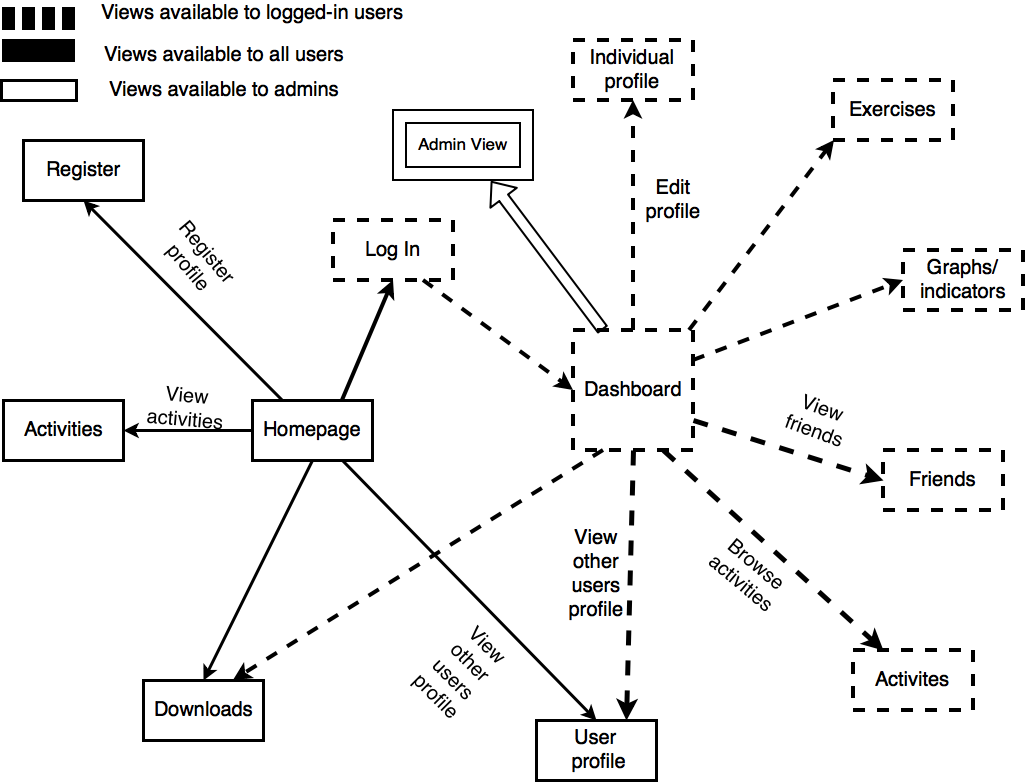
\includegraphics[scale=0.4]{Figures/StateDiagram.png}
\caption{State Diagram of Web Solution}
\label{fig:WebState}
\end{figure}


\subsection{State Diagram of Mobile App?}


\chapter{Test Strategy}
\section{Intro to Test Strategy}
\section{Formative Testing}
\section{Summative Testing}
\section{Usability Testing}
\section{Unit Testing}
\section{Integration Testing}
\section{Acceptance Test}
\section{Test Plan}
\section{Test Results}

\chapter{Evaluation of Solution}
\section{Requirements met}
\subsection{Functional}
Based on the unit tests which pass, we know which functional requirements are met:
Following is a list of the functional requirements of the system which are implemented and working: 
\begin{multicols}{3}
\begin{enumerate}
    \item FR1
    \item FR2
    \item FR3
    \item FR4
    \item FR6
    \item FR7
    \item FR8 N/A
    \item FR9
    \item FR10
    \item FR13
    \item FR15
    \item FR16
    \item FR17
    \item FR18
    \item FR19
\end{enumerate}
\end{multicols}

See Table \ref{table:funcReq} for a detailed description of the functional requirements.

\subsection{Non-functional}
//This section will be filled in in the final version of the report.
\textbf{Usability}
(Evaluate according to senior usability guidelines form pre-study??)
\section{Requirements not met}
\subsection{Functional}
Based on the unit tests which do not pass, we know which functional requirements that are not met in the final solution:  
\begin{enumerate}
    \item FR5
    \item FR11
    \item FR12
    \item FR14
\end{enumerate}
\subsection{Non-functional}
//This section will be filled in in the final version of the report.




\chapter{Future Improvements}



We feel that our project could grow to be something really great and important in the future. More and important functionality may be added to further improve the experience of using both the app and the website. Being a solution geared towards elderly people enforces a certain type of user interface. This applies to both the website and the app.


//This section will be expanded in the final version of the report based on the Known bugs listed in the appendix (this is an empty section in this version).
Where applicable, suggested solutions to he known bugs will also be included

\chapter{Evaluation of the Project/Lessons Learned}
\section{Project Management}
\subsection{Team Roles??}
\subsection{Time Management??}
\subsection{Attendance}
\subsection{Backlog and Task Management}
A lesson we clearly learned at the end of the project was to minimize where and how task management is done. 
To manage the product- and sprint backlogs we, initially, decided to use a spreadsheet in google docs and Trello. The spreadsheet were used to plan the sprints, break down tasks, do estimation and assignment, whereas, Trello was used to keep track of the progress of the tasks. However, the customer wanted us to use issues actively on gitHub. We then started using gitHub task management features in addition to our already existing methods for doing so. Instead of helping us, this simply led to confusing issues and team members not knowing where to go to find issues. Different team members used different channels to update their progress, and Trello was quickly abandoned by most.

The reason we did not use gitHub to manage our project completely, even after having it suggested by the customer, was that we did not want to add tasks relating to the report to our repository on gitHub. We believed it was in the customers interest to keep them separate. However, towards the end of the project, we realized that the customer thought we managed all our tasks and backlog through gitHub, and was surprised to learn that we had another system we used as well. We all agreed that this made it difficult for the product owner to keep track of what was going on. 

Had we known about all the task management features of gitHub at the start of the project, we see, in hindsight, that we should have simply managed our project through this one channel from the start. This insight into gitHub and how it also eased communications with the customer has been a great lessons from the project.
\section{Customer and Vague requirements??}
The team members were unfamiliar with Lean principles of development, and the biggest challenge initially was to understand this way of working. Expecting to quickly have established clear requirements to base our work on, it was difficult for the team to respond to what we, at the time, felt was an indecisive customer. We see in hindsight, that the customer's approach to the development process was one we were not familiar with. It took us several weeks to realize that we could and should be more proactive in coming up with solutions and that we were equally capable as the customer when it came to brainstorm solutions.

Had we realized this sooner, we could probably have had greater progress in a couple of sprints. Some of our placeholder items in the final solution might have been fully implemented, but this is in no way guaranteed as they were still dependent on factors outside our control. 

One example is the fitness indicator on our web site. Initially we believed we were going to collect data, do calculations and present this to the user. However, we were never able to settle with the customer which types of data should form the basis for any calculations.Later in the project, it became clear that Adapt, the research project we are a part of, where the ones making decisions about this data, but that they had not yet decided either what kind of data should be measured. Thus, even if we had been proactive is designing solutions for how to display the data, the functionality could not have been fully implemented as the product owner was not even made completely aware of the data to be collected and measured.

\section{Development Tools??}

\chapter{Conclusion}
//This chapter will be completed in the final version of the report

\bibliographystyle{plain}
\bibliography{references}

\addcontentsline{toc}{chapter}{Bibliography}

\appendix
\chapter{Risk Analysis}

\begin{figure}[H]
\centering
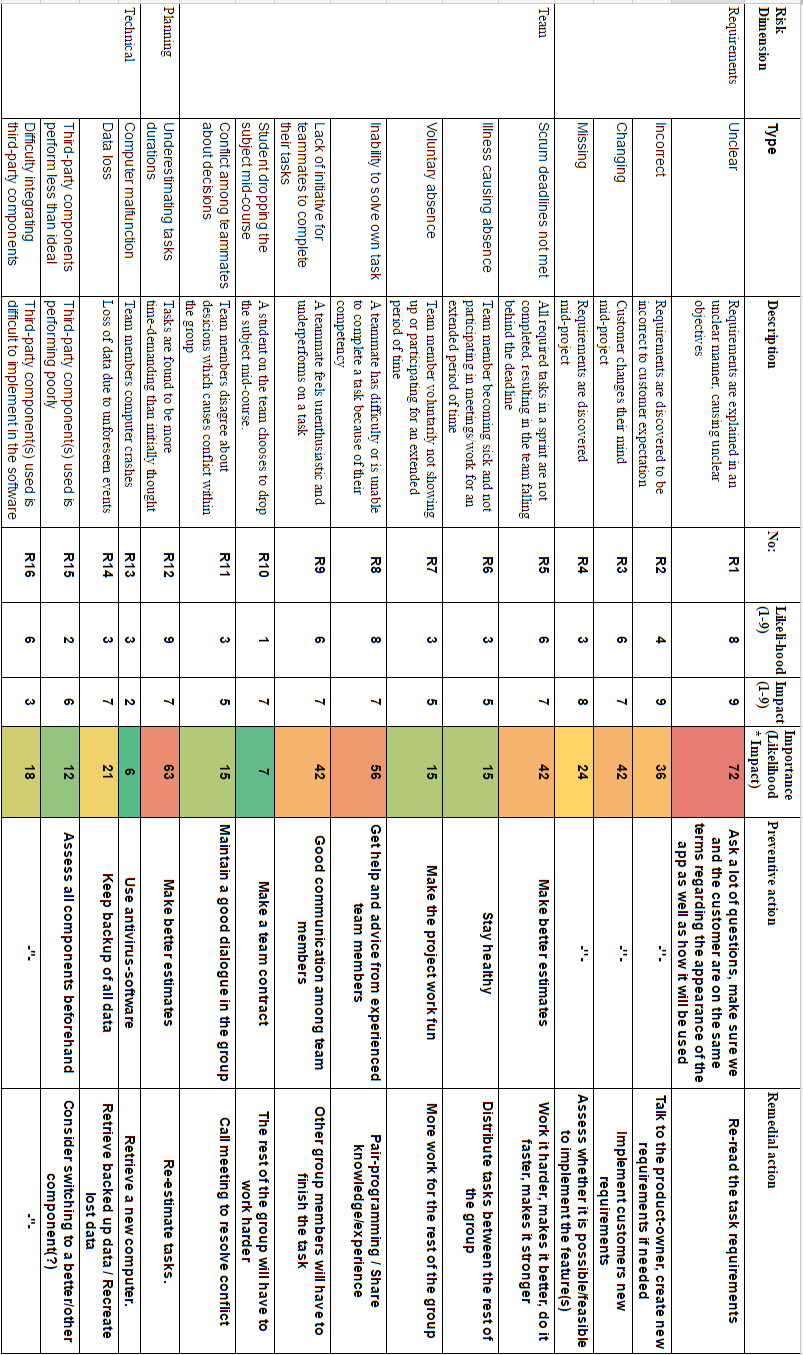
\includegraphics[scale=0.50]{Figures/riskMatrixBLA.png}
\caption{Risk Analysis}
\label{fig:RiskFull}
\end{figure}

\chapter{Sprints}
\section{Sprint 1}\label{sprint1}

\begin{figure}[H]
\centering
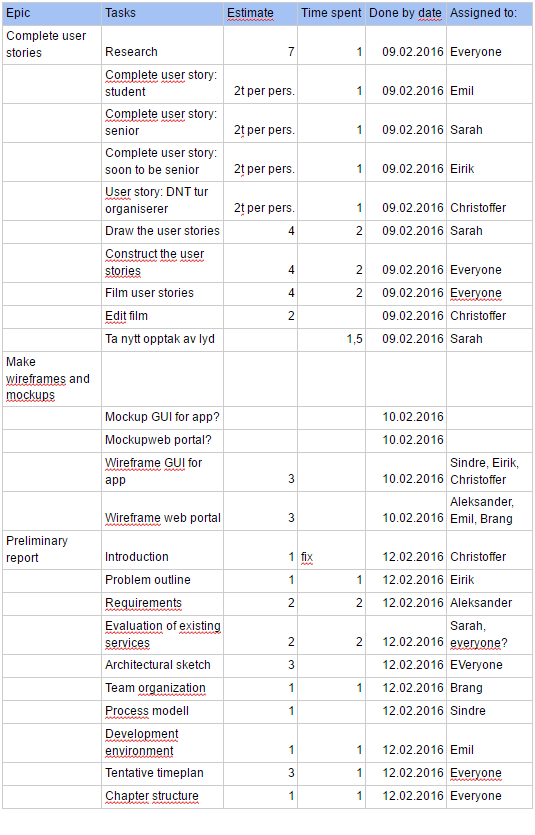
\includegraphics[width = 0.75\textwidth]{Figures/sprints/sprint1}
\caption{Sprint 1}
    \label{fig:SP1}
    \end{figure}

\section{Sprint 2}\label{sprint2}

\begin{figure}[H]
\centering
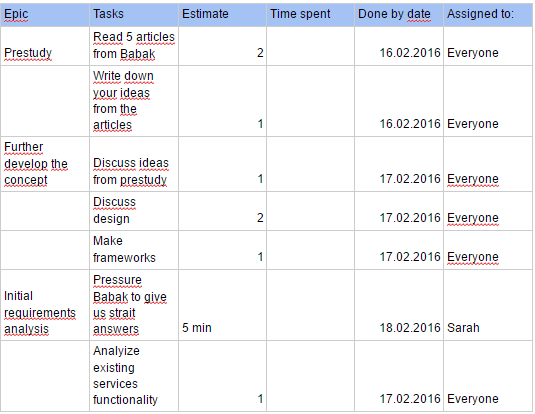
\includegraphics[width = 0.75\textwidth]{Figures/sprints/sprint2}
\caption{Sprint 2}
    \label{fig:SP2}
    \end{figure}

\section{Sprint 3}\label{sprint3}

\begin{figure}[H]
\centering
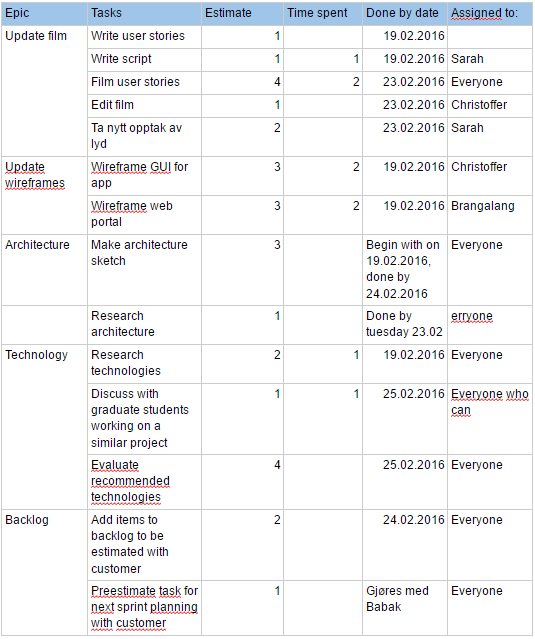
\includegraphics[width = 0.75\textwidth]{Figures/sprints/sprint3}
\caption{Sprint 3}
    \label{fig:SP3}
    \end{figure}

\section{Sprint 4}\label{sprint4}

\begin{figure}[H]
\centering
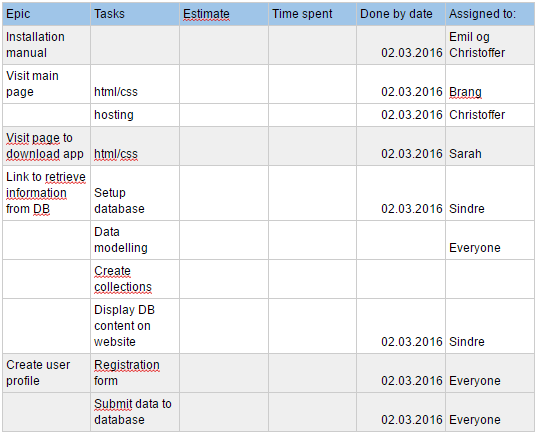
\includegraphics[width = 0.75\textwidth]{Figures/sprints/sprint4}
\caption{Sprint 4}
    \label{fig:SP4}
    \end{figure}

\section{Sprint 5}\label{sprint5}

\begin{figure}[H]
\centering
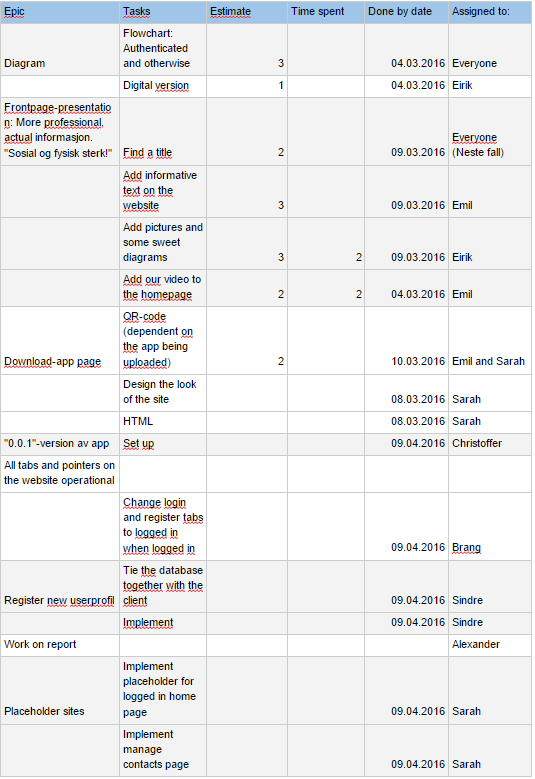
\includegraphics[width = 0.75\textwidth]{Figures/sprints/sprint5}
\caption{Sprint 5}
    \label{fig:SP5}
    \end{figure}

\section{Sprint 6}\label{sprint6}

\begin{figure}[H]
\centering
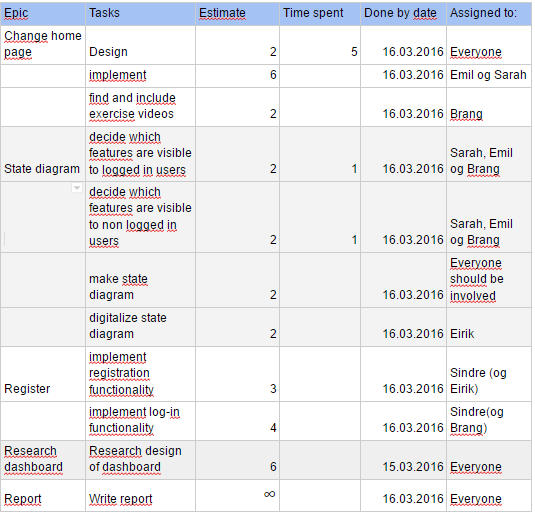
\includegraphics[width = 0.75\textwidth]{Figures/sprints/sprint6}
\caption{Sprint 6}
    \label{fig:SP6}
    \end{figure}

\section{Sprint 7}\label{sprint7}
The full sprint backlog for this sprint can be found on gitHub at \cite{sprint7}
\section{Sprint 8}\label{sprint8}
The full sprint backlog for this sprint can be found on gitHub at \cite{sprint8}
\section{Sprint 9}\label{sprint9}
The full sprint backlog for this sprint can be found on gitHub at \cite{sprint9}
\section{Sprint 10}\label{sprint10}
The full sprint backlog for this sprint can be found on gitHub at \cite{sprint10}


\chapter{Unit Tests}\label{unitTests}
\begin{table}[H]
\begin{tabular}{ | L{0.25\linewidth} | L{0.75\linewidth} | } 
 \hline \rowcolor{lightgray}
 Unit Test 1 &  \\
 \hline
 Test Item & Register user profile and log in as registered user \\ 
 \hline
 Test functional requirements no: & F1, F2
 \\ 
 \hline
 Approach & Register new user and log in with the provided details. \\ 
  \hline
 Item pass/fail criteria &  If webpage is not accessed, the test fails. If register does not work, the test fails, if login with the provided details from register does not work, the test fails. If users can register and log in with the provided details, the test passes. \\ 
 \hline
 Input &  Username, email and password\\ 
 \hline
 Expected results & Dashboard of the newly registered user \\ 
  \hline
Testing task & 
\vspace{-5mm}
    \begin{enumerate}[noitemsep]
  \item Enter website
  \item Click register
  \item Enter email and password
  \item Click log in and provide the same username, email and password
  \item Check if the user is logged in
   \end{enumerate}\\
 \hline
 Necessary environmental requirement & The website is running \\ 
 \hline
\end{tabular}
\caption{Unit test 1}
\end{table}

\begin{table}[H]
\begin{tabular}{ | L{0.25\linewidth} | L{0.75\linewidth} | } 
 \hline \rowcolor{lightgray}
 Unit Test 2 & \\
 \hline
 Test Item & User can edit their own profile information\\ 
 \hline
 Test functional requirements no: & F3
 \\
 \hline
 Approach & User can edit their profile information\\ 
  \hline
 Item pass/fail criteria &  If user clicks edit profile button, and nothing happens, the test fails. If the edited fields are not updated the test fails. If the user clicks edit, edits the fields and they are updated like expected, the test passes.\\ 
 \hline
 Input &  First name, last name, bio, password and profile picture\\ 
 \hline
 Expected results & Profile is edited successfully \\ 
  \hline
Testing task & 
\vspace{-5mm}
    \begin{enumerate}[noitemsep]
  \item User clicks edit profile
  \item User edits fields of their choice
  \item User clicks save
   \end{enumerate}\\
 \hline
 Necessary environmental requirement & The user is logged in and on the profile page\\ 
 \hline
\end{tabular}
\caption{Unit Test 2}
\end{table}

\begin{table}[H]
\begin{tabular}{ | L{0.25\linewidth} | L{0.75\linewidth} | } 
 \hline \rowcolor{lightgray}
 Unit Test 3 &  \\
 \hline
 Test Item & User can create event \\ 
 \hline
 Test functional requirements no: & F4
 \\
 \hline
 Approach & User clicks "createEvent" and fills in event form. Check if event shows up under "Mine aktiviteter" \\ 
  \hline
 Item pass/fail criteria &  If "createEvent" button is non-responsive, the test fails. If form cannot be filled in, the test fails. If event does not show ip in "Mine aktiviteter", the test fails. If event is displayed under "Mine aktiviteter", the test passes  \\ 
 \hline
 Input &  Any of the following: name, description, date, place, participants, type, difficulty level, public\\ 
 \hline
 Expected results & A newly created event displayed under "Mine aktiviteter" \\ 
  \hline
Testing task &
\vspace{-5mm}
    \begin{enumerate}[noitemsep]
  \item Click "Opprett ny aktivitet"
  \item Fill inn all fields of interest
  \item Submit form
  \item Check if event is displayed under "Mine aktiviteter"
   \end{enumerate}\\
 \hline
 Necessary environmental requirement & Successfully logged in to the user's account \\ 
 \hline
\end{tabular}
\caption{Unit test 3}
\end{table}

\begin{table}[H]
\begin{tabular}{ | L{0.25\linewidth} | L{0.75\linewidth} | } 
 \hline \rowcolor{lightgray}
 Unit Test 4 & \\
 \hline
 Test Item & Registered user can search for events\\ 
 \hline
 Test functional requirements no: & F5
 \\
 \hline
 Approach & Registered user can search for events\\ 
  \hline
 Item pass/fail criteria & If the user searches for an event and nothing happens, the test fails. If the user clicks the searched event and nothing happens, the test fails. If the user searches for an event, clicks the event, and is taken to "mine aktiviteter" displaying the chosen event.\\ 
 \hline
 Input &  The searched event\\ 
 \hline
 Expected results & The searched event is displayed \\ 
  \hline
Testing task & 
\vspace{-5mm}
    \begin{enumerate}[noitemsep]
  \item User searches for the event of their choice
  \item User clicks the searched event
   \end{enumerate}\\
 \hline
 Necessary environmental requirement & The user is logged in\\ 
 \hline
\end{tabular}
\caption{Unit Test 4}
\end{table}

\begin{table}[H]
\begin{tabular}{ | L{0.25\linewidth} | L{0.75\linewidth} | } 
 \hline \rowcolor{lightgray}
 Unit Test 5 & \\
 \hline
 Test Item & Registered user can invite friends to event\\ 
 \hline
 Test functional requirements no: & F6
 \\
 \hline
 Approach & User adds friend to event through dropdown menu\\ 
  \hline
 Item pass/fail criteria & If the user clicks "rediger denne aktiviteten" and nothing happens, the test fails. If the user clicks "klikk her for å legge til deltagere" and nothing happens, the test fails. If the user clicks "ferdig" and nothing happens, the test fails. If the user successfully edits the event and add users to the event, the test passes.\\ 
 \hline
 Input &  Searching and adding users\\ 
 \hline
 Expected results & New event with the selected users added to the participant list \\ 
  \hline
Testing task &
\vspace{-5mm}
    \begin{enumerate}[noitemsep]
  \item User clicks "rediger denne aktiviteten" which brings up the modal for editing the event
  \item User clicks "klikk her for å legge til deltagere" and types in the user it wants add and selects it
  \item User clicks "ferdig"
   \end{enumerate}\\
 \hline
 Necessary environmental requirement & The user is logged in and is in "mine aktivteter" and has clicked the event of their choice\\ 
 \hline
\end{tabular}
\caption{Unit Test 5}
\end{table}

\begin{table}[H]
\begin{tabular}{ | L{0.25\linewidth} | L{0.75\linewidth} | } 
 \hline \rowcolor{lightgray}
 Unit Test 6 &  \\
 \hline
 Test Item & Registered user can join other users events\\ 
 \hline
 Test functional requirements no: & F7
 \\ 
 \hline
 Approach & User receives invitation to event, click on it and can choose between "Accept" and "Decline" \\ 
  \hline
 Item pass/fail criteria &  If user cannot see any buttons for "Accept" and "Decline", the test has failed. If the user accepts of declines the invitation, but their status is not updated in eventDetails, the test fails. If the user's status is updated, the test passes  \\ 
 \hline
 Input &  Click on "Accept"/"Decline"\\ 
 \hline
 Expected results & Status updated in event details view \\ 
  \hline
Testing task & 
\vspace{-5mm}
    \begin{enumerate}[noitemsep]
  \item Click on the event invitation
  \item Click on "Accept" or "Decline"
  \item Check if status is updated in event details view.
   \end{enumerate}\\
 \hline
 Necessary environmental requirement & Successfully logged in to the user's account \\ 
 \hline
\end{tabular}
\caption{Unit test 6}
\end{table}


\begin{table}[H]
\begin{tabular}{ | L{0.25\linewidth} | L{0.75\linewidth} | } 
 \hline \rowcolor{lightgray}
 Unit Test 7 &  \\
 \hline
 Test Item & Non-registered user can view public events\\
 \hline
 Test functional requirements no: & F8
 \\
 \hline
 Comment & This requirement was removed\\
 \hline
\end{tabular}
\caption{Unit test 7}
\end{table}

\begin{table}[H]
\begin{tabular}{ | L{0.25\linewidth} | L{0.75\linewidth} | } 
 \hline \rowcolor{lightgray}
 Unit Test 8 &  \\
 \hline
 Test Item & Registered user can view their fitness information in his/her profile page\\ 
 \hline
 Test functional requirements no: & F9
 \\ 
 \hline
 Approach & User is able to view the placeholder data fields that we use for this requirement\\ 
  \hline
 Item pass/fail criteria &  If user clicks the admin tab and nothing happens, the test fails. If the user click the admin tab and is taken to the admin view, the test passes.\\ 
 \hline
 Input & User clicks on the admin tab\\ 
 \hline
 Expected results & User is able to view placeholders\\ 
  \hline
Testing task & 
\vspace{-5mm}
    \begin{enumerate}[noitemsep]
  \item[] This requirement is done with placeholders and these are placed in the admin view.
  \item User clicks on admin tab
   \end{enumerate}\\
 \hline
 Necessary environmental requirement & User is logged in and is an admin\\ 
 \hline
\end{tabular}
\caption{Unit test 8}
\end{table}

\begin{table}[H]
\begin{tabular}{ | L{0.25\linewidth} | L{0.75\linewidth} | } 
 \hline \rowcolor{lightgray}
 Unit Test 9 &  \\
 \hline
 Test Item & Registered user can manually add their activities \\ 
 \hline
 Test functional requirements no: & F10
 \\ 
 \hline
 Approach & User manually adds an activity through activity page\\
  \hline
 Item pass/fail criteria & If the "finn nye øvelser og aktiviteter" button does not work, the test fails. If any of the "balanse", "styrke" and "fleksibilitet" buttons do not work, the test fails. If the user cannot select an exercise, the test fails. If the button "legg til i mine øvelser" does not work, the test fails. If the user successfully adds an activity the test passes.\\
 \hline
 Input &  Select activity and add activity of your choice\\ 
 \hline
 Expected results & Activity added under "dine øvelser" on your dashboard \\ 
  \hline
Testing task & 
\vspace{-5mm}
    \begin{enumerate}[noitemsep]
  \item User clicks "finn nye øvelser og aktiviteter"
  \item User sorts by "balanse", "styrke" and "fleksibilitet"
  \item User selects the exercise they want to add to their profile
  \item User clicks the button labeled "legg til i mine øvesler"
   \end{enumerate}\\
 \hline
 Necessary environmental requirement & The user is logged in and is in the activities page \\ 
 \hline
\end{tabular}
\caption{Unit test 9}
\end{table}

\begin{table}[H]
\begin{tabular}{ | L{0.25\linewidth} | L{0.75\linewidth} | } 
 \hline \rowcolor{lightgray}
 Unit Test 10 &  \\
 \hline
 Test Item & Registered user can search for and view other users' profiles \\ 
 \hline
 Test functional requirements no: & F11
 \\ 
 \hline
 Approach & User searches for a user and views their profile\\
  \hline
 Item pass/fail criteria & If the user cannot initiate a search, the test fails. If the user cannot use the search bar to search, the test fails. If a user cannot click another user and view their profile, the test fails. If a user is able to use the search bar, which leads to being able to view another users profile, the test passes.\\
 \hline
 Input &  Name of the user' profile you want to view\\ 
 \hline
 Expected results & Have a view of the user' profile of your choice\\ 
  \hline
Testing task & 
    \vspace{-5mm}
    \begin{enumerate}[noitemsep]
  \item User clicks the search bar to initiate a search
  \item User searches for a user of their choice
  \item User clicks the user they have searched for
   \end{enumerate}\\
 \hline
 Necessary environmental requirement & The user is logged in and is on the dashboard\\ 
 \hline
\end{tabular}
\caption{Unit test 10}
\end{table}

\begin{table}[H]
\begin{tabular}{ | L{0.25\linewidth} | L{0.75\linewidth} | } 
 \hline \rowcolor{lightgray}
 Unit Test 11 &  \\
 \hline
 Test Item & Registered user can view friend list\\
 \hline
 Test functional requirements no: & F12
 \\ 
 \hline
 Approach & User clicks a button to view their friend list\\
  \hline
 Item pass/fail criteria & If the user clicks "kontakter" and the button is unresponsive, the test fails. If the user clicks "kontakter" and it directs you to your friend list, the test passes.\\
 \hline
 Input &  Click on the "kontakter" button\\ 
 \hline
 Expected results & View your friend list\\
  \hline
Testing task &
    \vspace{-5mm}
    \begin{enumerate}[noitemsep]
  \item User clicks the button labeled "kontakter" 
   \end{enumerate}\\
 \hline
 Necessary environmental requirement & The user is logged in and is on the dashboard\\ 
 \hline
\end{tabular}
\caption{Unit test 11}
\end{table}

\begin{table}[H]
\begin{tabular}{ | L{0.25\linewidth} | L{0.75\linewidth} | } 
 \hline \rowcolor{lightgray}
 Unit Test 12 &  \\
 \hline
 Test Item & Registered user can add/delete friends from friend list\\
 \hline
 Test functional requirements no: & F13
 \\
 \hline
 Approach & User navigates to the user of their choice and adds/deletes them from their friend list\\
  \hline
 Item pass/fail criteria & If the user clicks "kontakter" and the button is unresponsive, the test fails. If the user clicks "kontakter" and it directs you to your friend list, the test passes.\\
 \hline
 Input &  Click on the "kontakter" button, click the "legg til venn" button, click a username, click unfriend button\\ 
 \hline
 Expected results & The user has either added or deleted a contact\\
  \hline
Testing task &
    \vspace{-5mm}
    \begin{enumerate}[noitemsep]
  \item User clicks the button labeled "kontakter"
  \item User selects the "legg til venn" button next to the user they wish to add
  \item User clicks the the username of the contact they wish do delete
  \item User clicks the unfriend button
   \end{enumerate}\\
 \hline
 Necessary environmental requirement & The user is logged in and is on the dashboard\\ 
 \hline
\end{tabular}
\caption{Unit test 12}
\end{table}

\begin{table}[H]
\begin{tabular}{ | L{0.25\linewidth} | L{0.75\linewidth} | } 
 \hline \rowcolor{lightgray}
 Unit Test 13 &  \\
 \hline
 Test Item & Registered users can instant message other users\\
 \hline
 Test functional requirements no: & F14
 \\
 \hline
 Approach & User find the user they want to instant message and sends them a message\\
  \hline
 Item pass/fail criteria & If the user clicks "send melding" and nothing happens, the test fails. If the user types in a username and nothing happens, the test fails. If the user clicks "send melding" and types in the username of their choice, and manages to send an instant message, the test passes.\\
 \hline
 Input &  Click on the "send message" button, type in the username of the user you want to instant message, click the "send" button\\ 
 \hline
 Expected results & The user has sent an instant message to another user\\
  \hline
Testing task &
    \vspace{-5mm}
    \begin{enumerate}[noitemsep]
  \item User clicks the button labeled "Send melding"
  \item User types in the name of the user they want to instant message and selects it
  \item User types in the message the want to send and clicks send
   \end{enumerate}\\
 \hline
 Necessary environmental requirement & The user is logged in and is on the dashboard, also must be friends with the user they want to instant message\\
 \hline
\end{tabular}
\caption{Unit test 13}
\end{table}

\begin{table}[H]
\begin{tabular}{ | L{0.25\linewidth} | L{0.75\linewidth} | } 
 \hline \rowcolor{lightgray}
 Unit Test 14 &  \\
 \hline
 Test Item & All users should be able to download the app from the website\\
 \hline
 Test functional requirements no: & F15
 \\
 \hline
 Approach & User downloads the app from the website by clicking the app store that corresponds with their smartphone/tablet\\
  \hline
 Item pass/fail criteria & If the user clicks "Last ned til din mobil" tab, and nothing happens, the test fails. If the user clicks either of the app store buttons in the footer and nothing happens, the test fails. If the user clicks either the "Last ned til din mobil" tab or one of the app stores in the footer and they are able to download the app successfully, the test passes.\\
 \hline
 Input & Click on the "Last ned til din mobil" tab, click on the app store of your choice\\ 
 \hline
 Expected results & The user successfully downloads the app\\
  \hline
Testing task &
    \vspace{-5mm}
    \begin{enumerate}[noitemsep]
  \item User clicks can either click the "Last ned til din mobil" tab on the website homepage or click the the button corresponding to the platform of their choice under "Last ned appen til din mobil" in the footer
  \item If the user click the "Last ned til din mobil" tab, the user can pick the button to download from either app store or google play
   \end{enumerate}\\
 \hline
 Necessary environmental requirement & The user can be logged in or not\\
 \hline
\end{tabular}
\caption{Unit test 14}
\end{table}

\begin{table}[H]
\begin{tabular}{ | L{0.25\linewidth} | L{0.75\linewidth} | } 
 \hline \rowcolor{lightgray}
 Unit Test 15 &  \\
 \hline
 Test Item & All users should be able to view different exercises on the web page\\
 \hline
 Test functional requirements no: & F16
 \\
 \hline
 Approach & User clicks the "se alle øvelser" button to view all the different exercises\\
  \hline
 Item pass/fail criteria & If the user clicks "se alle øvelser" button, and nothing happens, the test fails. If the user clicks "se alle øvelser" button, and is able to see all the exercises, the test passes.\\
 \hline
 Input & Click on the "se alle øvelser" button\\ 
 \hline
 Expected results & The user successfully views the different exercises on the web page\\
  \hline
Testing task &
    \vspace{-5mm}
    \begin{enumerate}[noitemsep]
  \item User clicks on the "se alle øvelser" button
   \end{enumerate}\\
 \hline
 Necessary environmental requirement & The user has to be logged in and be on the dashboard\\
 \hline
\end{tabular}
\caption{Unit test 15}
\end{table}

\begin{table}[H]
\begin{tabular}{ | L{0.25\linewidth} | L{0.75\linewidth} | } 
 \hline \rowcolor{lightgray}
 Unit Test 16 & \\
 \hline
 Test Item & All users should be able to take a simple fitness test on the web site\\
 \hline
 Test functional requirements no: & F17
 \\
 \hline
 Approach & User fills out and takes the fitness test\\
  \hline
 Item pass/fail criteria & If the user clicks the "Hva er din fysiske alder?" button and it does nothing, the test fails. If the user is unable to fill in the information required to take the fitness test, the test fails. If the user is able to get to and take the fitness test, the test passes.  \\
 \hline
 Input & Click the "Hva er din fysiske alder?" button and fill in the required info\\ 
 \hline
 Expected results & The user successfully take the fitness test\\
  \hline
Testing task &
    \vspace{-5mm}
    \begin{enumerate}[noitemsep]
  \item User clicks on the button called "Hva er din fysiske alder?"
  \item User fills in the information needed to take the test
   \end{enumerate}\\
 \hline
 Necessary environmental requirement & The website is up and running\\
 \hline
\end{tabular}
\caption{Unit test 16}
\end{table}

\begin{table}[H]
\begin{tabular}{ | L{0.25\linewidth} | L{0.75\linewidth} | } 
 \hline \rowcolor{lightgray}
 Unit Test 17 &  \\
 \hline
 Test Item & Registered users should get updates from other users in a news feed\\
 \hline
 Test functional requirements no: & F18
 \\
 \hline
 Approach & User can view updates from other users in their news feed\\
  \hline
 Item pass/fail criteria & If the user is unable to view other users event in their news feed, the test fails. If the user is able to view other users event in their news feed, the test passes.\\
 \hline
 Input & Viewing posts in the newsfeed requires no input, when you already are on the dashboard\\ 
 \hline
 Expected results & The user successfully\\
  \hline
Testing task &
    \vspace{-5mm}
    \begin{enumerate}[noitemsep]
  \item[] (User performs any action, like adding a friend, creating or attending an event, which will show up in the newsfeed)
  \item User 1 creates a public event
  \item User 2 can view the newly created event on the in the newsfeed on the dashboard
   \end{enumerate}\\
 \hline
 Necessary environmental requirement & The user is logged in and on the dashboard\\
 \hline
\end{tabular}
\caption{Unit test 17}
\end{table}

\begin{table}[H]
\begin{tabular}{ | L{0.25\linewidth} | L{0.75\linewidth} | } 
 \hline \rowcolor{lightgray}
 Unit Test 18 &  \\
 \hline
 Test Item & All users should be able to get basic information about fall risk\\
 \hline
 Test functional requirements no: & F19
 \\
 \hline
 Approach & User reads about fall risk on the website\\
  \hline
 Item pass/fail criteria & If the user is unable to get information about fall risk, the test fails. If the user is able to get information about fall risk, the test passes.\\
 \hline
 Input & Nope.\\ 
 \hline
 Expected results & The user is able to get information about fall risk\\
  \hline
Testing task &
    \vspace{-5mm}
    \begin{enumerate}[noitemsep]
  \item The user scrolls down on the website homepage and reads about fall risk
   \end{enumerate}\\
 \hline
 Necessary environmental requirement & The website is up and running and the user is on the website\\
 \hline
\end{tabular}
\caption{Unit test 18}
\end{table}

//We will add unit tests for the additional requirements in the final version of the report

\chapter{Known Bugs}

\textit{Here we will list known bugs at the time of delivery}

\end{document}
